\setcounter{chapter}{1}
\setcounter{equation}{0}
\addcontentsline{toc}{chapter}{Глава 1. Алгоритм оценки информационных параметров для одного источника сигнала в CDMA-системах на фоне АБГШ}
\chapter*{Глава 1. Алгоритм оценки информационных параметров для одного источника сигнала в CDMA-системах на фоне АБГШ}

\section{Постановка задачи}
В первой главе рассмотрена система передачи информации (СПИ) с расширенным спектром методом прямой последовательности. Приведены основные свойства и характеристики
таких систем. Рассмотрены источники помех и оптимальный в смысле максимального правдоподобия приемник для CDMA-системы Navstar GPS. В данной главе ставится и решается задача синтеза  
алгоритма оценки информационных параметров ШПС на основе авторегрессионной модели сигнала для одного источника на фоне АБГШ. Точность оценки приведенного алгоритма сравнивается с границей Крамера-Рао. 

Объектом исследования являются приемники типового широкополосного сигнала - СНС Navstar GPS.
Сигнал данной системы был выбран по причине относительно простой возможности к его доступу (сбору сигнала, а также наличию уже собранного сигнала в общедоступных источниках) и широкого распространения.
Основные модули этой системы изображены на \mbox{Рис. \ref{pic:sec1_gnss_system}.}
\begin{figure}[h]
	\center\scalebox{1}{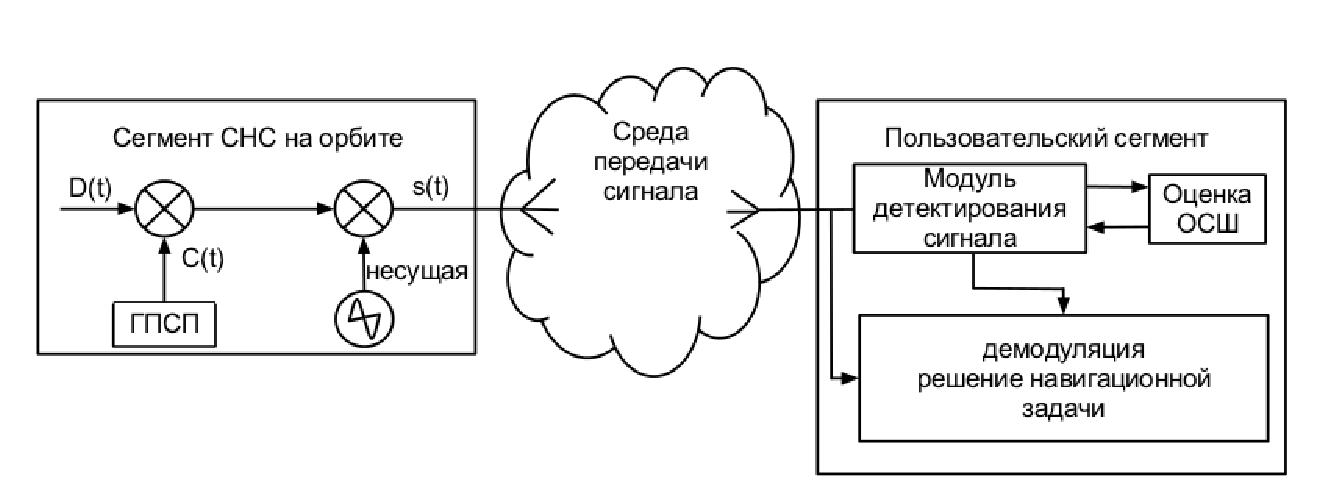
\includegraphics[width=1\linewidth]{sec1gnss_system.eps}}
	\caption{Структурная схема СНС GPS}
	\label{pic:sec1_gnss_system}
\end{figure}
В систему СНС Navstar GPS входят космический сегмент, наземный сегмент (на Рис. \ref{pic:sec1_gnss_system} не
отражен), а также пользовательский сегмент. В космический сегмент входит спутниковая группировка, в 
наземный - станции управления, в пользовательский - все устройства принимающие, сигнал от СНС Navstar GPS.

%В системе СНС Navstar GPS применяется ШПС. Система передачи информации считается системой с расширенным спектром в следующих случаях \cite{sklyar}:
%\begin{enumerate}
%	\item Используемая полоса значительно шире минимальной, необходимой для передачи данных.
%	\item Расширение спектра производится с помощью так называемого расширяющего сигнала (ПСП),
%		который не зависит от передаваемой информации.
%	\item Восстановление исходных данных ("сужение спектра") осуществляется путем сопоставления полученного
%		сигнала и синхронизированной копии расширяющего сигнала (ПСП)
%\end{enumerate}
%
%Так же подобные сигналы называют:
%\textquotedblleftсложными\textquotedblright,
%\textquotedblleftшумоподобными\textquotedblright,
%\textquotedblleftпсевдослучайными\textquotedblright,
%\textquotedblleftсложными-дискретными\textquotedblright,
%\textquotedblleftдискретно-кодированными\textquotedblright,
%\textquotedblleftортогональными (квазиортогональными)\textquotedblright,
%\textquotedblleftоптимальными дискретными\textquotedblright
%\cite{gantmaher-book}.
%
%Каждое название ставит акцент на определенной характеристике сигнала. В данной работе я буду оперировать термином
%широкополосный сигнал - ШПС. ШПС можно определить, как \cite{gantmaher-book, varakin-book}:
%\begin{equation}
%	\label{eq:ss_signal}
%	1 << FT = B,
%\end{equation}
%где ${B}$ - база сигнала, ${F}$ - эффективная ширина спектра, а ${T}$ - длительность.
%Неточность этого определения рассмотрена в \cite{gantmaher-book}, также там даны ссылки на другие источники
%разделяющие критику данного определения. Для данной работы критика, рассмотренная в приведенных источниках,
%принципиального значения не имеет.

Рассматривается сигнал с расширением спектра методом "прямой последовательности".
Данный метод заключается в том, что гармоническая несущая сигнала модулируется высокоскоростным (широкополосным)
расширяющим сигналом. 

Несущее колебание с частотой ${\omega_0}$  модулируется данными ${d(t)}$, а также высокоскоростной ПСП ${g(t)}$, полученной методом "прямой последовательности".
В СПИ Navstar GPS осуществляется двоичная фазовая модуляция (ДФМ или 2-ФМ), а значит ${d(t)}$  и ${g(t)}$  - потоки антиподных импульсов \{-1, 1\}.
На \mbox{Рис. \ref{pic:bit_and_code}} представлены: фрагмент цифровых данных и модулирующей последовательности на длине 1-го бита ${T_b}$.
\begin{figure}[h]
	\center\scalebox{0.5}{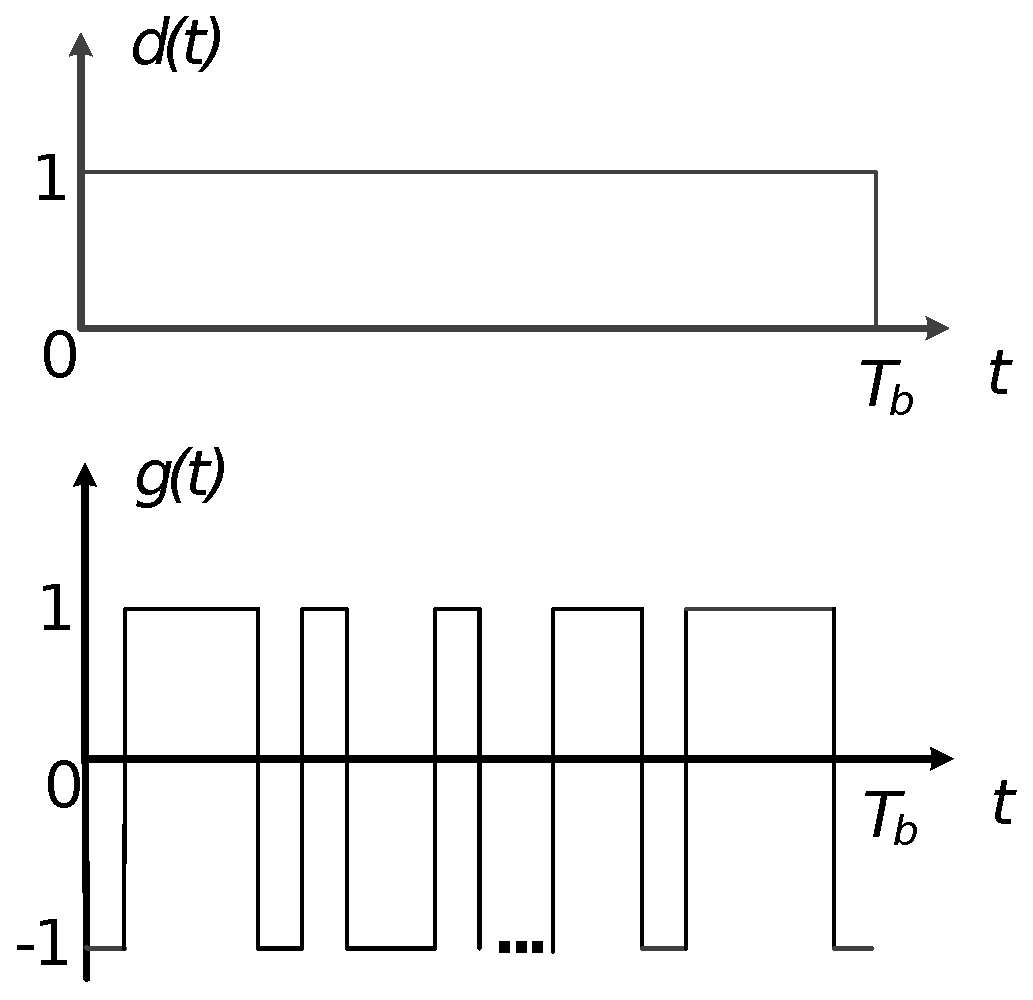
\includegraphics[width=1\linewidth]{bit_and_code.eps}}
	\caption{Информационный бит ${d(t)}$ и модулирующая последовательность ${g(t)}$ } 
	\label{pic:bit_and_code}
\end{figure}

Таким образом сигнал на выходе модулятора может быть представлен \cite{shahtarin_sync}:
\begin{equation}
	\label{eq:cdma_eq}
	s(t)=Ad(t)g(t)\cos{(\omega_{0}t)},
\end{equation}
где ${A}$ - амплитуда, ${d(t)}$- информационный бит, а ${g(t)}$ - ПСП.

Как уже было отмечено при данном методе
расширение спектра достигается за счет модуляции несущей частоты чаще всего двоичной ПСП или за счет псевдослучайной перестройки рабочей частоты \cite{borisovBook}.
Рассматриваемое в работе семейство ПСП Голда относится к ПСП, модулирующей сигнал при помощи псевдослучайной перестройки фазы - фазо-манипупулированный широкополосный сигнал
(ФМШПС). Так как в данной работе не рассматриваются другие виды ПСП, будем заменять термин ФМШПС термином ШПС, принимая во внимание только случай ФМШПС.

Таким образом (\ref{eq:cdma_eq}) может быть также записано как:
\begin{equation}
	\label{eq:cdma_eq_phi}
	s(t)=Ad(t)\cos{(\omega_{0}t + \theta_k)},
\end{equation}
где ${(\theta_k=\alpha_k \pi, \alpha_k \in \{0, 1\})}$.

Амплитуда ${A}$ сигнала зависит от многих факторов и должна рассматриваться как случайная величина \cite{pestryakov-book}. Случайность
амплитуды может иметь разный характер. Обычно амплитуда сигнала неизвестна и может изменяться в широких пределах,
но очень медленно, в зависимости от условий функционирования системы. Большой интерес представляет определение пороговых
значений мощности (амплитуды) или энергии сигнала при заданном уровне помех, обеспечивающих при оптимальном
обнаружении требующуюся достоверность обнаружения или передачи сообщения. В этих условиях амплитуду сигнала или его энергию
полезно рассматривать как переменную величину и исследовать ее влияние на результат работы системы.

Информационный бит ${d(t)}$ остается постоянным в течении промежутка ${T_b}$:
\begin{equation}
	\label{eq:cdma_eq_data}
	 d(t) = \begin{cases}
		1, 0 \le t \le T_b; \\
		0, t \not\in [0, T_b].
		\end{cases}
\end{equation}

В случае прямоугольной формы символов информационной последовательности двоичной ШПС на длительности одного бита данных, сигнал можно представить как:
\begin{equation}
	\label{eq:cdma_eq_phi}
	s(t)=Ad(t)g(t)\cos{(\omega_{0}t + \theta_0)}, 0 \le t \le T_b,
\end{equation}
где ${\theta_0}$ - начальная фаза сигнала, ее значение имеет равномерное распределение на интервале ${(\theta_0 \in [0, 2\pi])}$.

Известно, что для случайной последовательности (СП) корреляционная функция (КФ) равна:
\begin{equation}
	\label{eq:cdma_ca_corr_func}
	 R_p(\tau) = \begin{cases}
		1 - \frac{|\tau|}{\tau_c}, |\tau| < \tau_c; \\
		0, |\tau| > \tau_c.
		\end{cases}
\end{equation}

График КФ СП приведен на Рис. \ref{pic:cf_code}.
\begin{figure}[h]
	\center\scalebox{0.7}{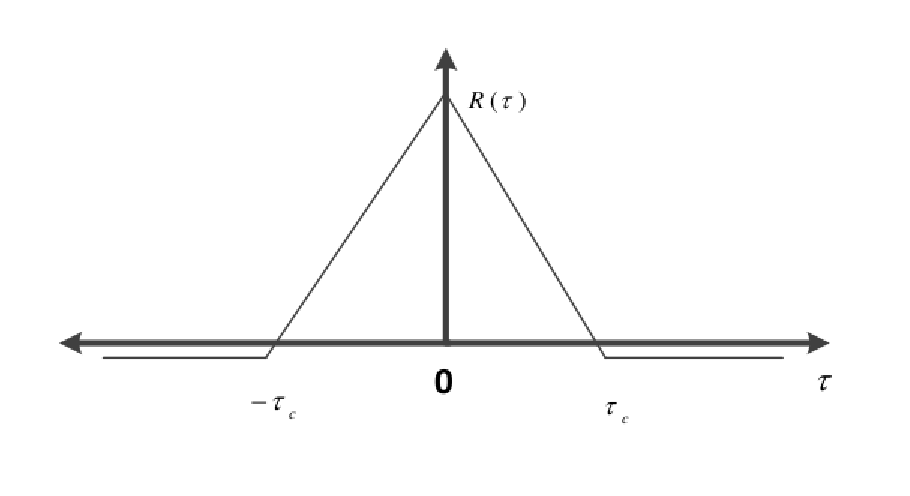
\includegraphics[width=1\linewidth]{cf_code.eps}}
	\caption{График КФ СП} 
	\label{pic:cf_code}
\end{figure}

СПМ ${G_p(f)}$ центрированного СП по теореме Винера-Хинчина является преобразованием Фурье
от КФ \cite{borisovBook}:
\begin{align}
	\label{eq:psd_corr_func}
	G_p(f) & = & \int^{\inf}_{inf} R(\tau)e^{-j2\pi f \tau} d\tau = \int^{\inf}_{inf} \left( 1 - \frac{|\tau|}{\tau_c} \right) e^{-j2\pi f \tau} d\tau = \nonumber \\
		& = & \int^{\tau_c}_{0}\left( 1 - \frac{|\tau|}{\tau_c} \right) \cos{(2\pi f \tau)} d\tau = \tau_c \left( \frac{\sin{(\pi f \tau_c)}}{\pi f \tau_c} \right)^2.
\end{align}

Выражение (\ref{eq:psd_corr_func}) представляет собой СПМ произведения ${p(t)d(t)}$ при использовании случайного сигнала ${p(t)}$.

Из литературы по теории автоматических систем, например, \cite{pugachev}, известна классическая постановка
задачи теории оптимальных систем. "На практике часто приходится решать задачу проектирования системы, когда
требуется определить характеристики системы таким образом, чтобы она имела наибольшую точность при данных условиях.
Систему, обеспечивающую наибольшую возможную точность с какой-нибудь определенной точки зрения среди всех систем
заданного класса, обычно называют оптимальной" \cite{pugachev}.

В одной из постановок данной задачи \cite{pugachev}, система считается полностью неизвестной
и требуется определить ее оператор так, чтобы она была оптимальной с точки зрения принятого критерия качества. Эта
задача сводится к определению с наибольшей возможной точностью некоторых параметров, от которых зависит принимаемый
сигнал. Но при этом важно учитывать не только точность, но и другие факторы, так как проектируемая система должна
удовлетворять многим, часто противоречивым требованиям. В виду приведенных факторов, обычно представляет собой
ряд компромиссных решений, удовлетворяющих всем предъявляемым к системе требованиям.

Точность автоматической системы обычно характеризуется математическим ожиданием и дисперсией ее ошибки.
Математическое ожидание представляет собой систематическую ошибку системы в данных условиях, а дисперсия
характеризует уровень случайных ошибок \cite{pugachev}. Так как в различных условиях работы
системы, которые встречаются случайно, систематическая ошибка тоже является случайной, за критерий качества
системы при ее проектировании обычно принимают второй начальный момент ошибки - математическое ожидание
квадрата ошибки:
\begin{equation}
	\label{eq:stat_err_prob}
	\eta = M[e^2(t)].
\end{equation}

Положительный квадратный корень из этой величины называют средней квадратической ошибкой  (СКО) системы. Таким образом,
оптимальной системой обычно считают такую систему, которая имеет минимальную среднюю квадратичную ошибку.

Критерий минимума СКО является простейшим с математической точки зрения и обычно приводит
к наиболее простым методам определения оптимальных систем. Следует отметить, что далеко не во всех задачах он может служить мерой
качества системы. 

В случаях, когда необходимо проектировать следящую систему, приходится учитывать возможность срыва слежения,
который заключается в том, что система перестает работать, если ее ошибка превосходит по абсолютной величине некоторый
уровень. При проектировании таких систем целесообразно принять за критерий качества вероятность срыва слежения. При
этом оптимальной считается такая система, которая обеспечивает минимум вероятности срыва слежения. Если срыв слежения
происходит в случае, когда абсолютная величина ошибки превосходит уровень $a$, то критерий минимума вероятности ошибки
слежения можно представить \cite{pugachev} (глава 10.2):
\begin{equation}
	\label{eq:prob_lost_signal}
	p = P(e(t) > a) = \mbox{min}.
\end{equation}

Оценка параметров сигнала всегда происходит в условиях действия помех и, решая задачу оптимизации приема,
необходимо иметь в виду определенные модели помех. Основной помехой является флуктуационная с нормальным
распределением мгновенных значений и широким равномерным энергетическим спектром. Такие помехи характеризуются
плотностью мощности ${\sigma_n^2}$ на входе схемы обработки \cite{pestryakov-book}.

Вторым видом помех, оказывающих
большое влияние на прием сигналов, являются помехи, связанные с рассеянным или многолучевым распространением
радиосигналов. Многолучевое распространение радиоволн можно рассматривать двояко: или как фактор, обуславливающий
наличие дополнительных помех в виде сигналов, аналогичных тому, который рассматривается как основной, но с другой
задержкой; или как фактор изменяющий статистические характеристики параметров принимаемого сигнала,
обуславливая случайность амплитуды \cite{pestryakov-book}.

Третьим видом помех, характерных для систем связи, использующих ШПС, являются помехи от шумоподобных сигналов,
принадлежащих другим адресам (каналам). Эти помехи определяются тем, что при использовании ШПС для разделения
сигналов по форме (кодовое разделение) сигналы, принадлежащие другим адресам, не являясь идеально ортогональными,
создают помехи. Сумма нескольких шумоподобных сигналов дает результирующий процесс, близкий к нормальному шуму,
поэтому помеху, создаваемую многими ШПС, почти всегда можно рассматривать как нормальный шум с ограниченным
равномерным спектром и ограниченной мощностью \cite{pestryakov-book}.

Мощность АБГШ подвергается значительным изменениям. Это обусловлено
изменением собственных шумов приемника, помехами, создаваемыми атмосферой и космосом, усилением приемного устройства
и т.п. Следовательно, для АБГШ плотность мощности ${N_n}$ является случайной величиной.

В системе Navstar GPS можно выделить 6 источников помех \cite{parkinson_1996}:
\begin{itemize}
	\item {данные эфемерид - ошибки в позициях спутников;}
	\item {часы спутника - ошибки в переданных данных о времени;}
	\item {ионосфера - ошибки в коррекции псевдодальностей, обусловленных ионосферными эффектами;}
	\item {тропосфера - ошибки в коррекции псевдодальностей, обусловленных тропосферными эффектами;}
	\item {многолучевость - эффект отраженных сигналов, принятых антенной;}
	\item {приемник - ошибки в измерениях обусловленные термальным шумом, точностью программного обеспечения (ПО) и т.д.}
\end{itemize}

Так как данные виды помех влияют только на точность определения координат, мы можем рассматривать упрощенную модель
канала, где данные виды помех не рассматриваются отдельно. В данной работе рассмотрены помехи, обусловленные интерференционной помехой и АБГШ. 
Более углубленные модели канала можно найти в
источниках: упрощенная модель канала с сигналом на промежуточной частоте \cite{lei_dong_phd}, модель многолучевого
распространения \cite{hannah_phd}, а также \cite{burns_model, corbell_model, brown_model}.

\section{Алгоритм оптимальной оценки параметров ШПС}
Алгоритм реализующий метод максимального правдоподобия - последовательный коррелятор. Данный подход реализуется в аппаратных приемниках.
Аппаратный приемник позволяет реализовать параллельно несколько последовательных корреляторов и вести оценку параметров
СПИ с ШПС параллельно.

Данный алгоритм в некоторых источниках также называется согласованным фильтром. В \cite{sklyar} рассмотрены нюансы этих двух понятий.
В данной работе используется понятие последовательный коррелятор. Работа коррелятора описывается математической операцией
корреляции:
\begin{equation}
	\label{eq:serial_corr}
	y(m)=\sum\limits_{n=0}^{N-1}{x(n)h(m+n)},
\end{equation}
где ${x(n)}$ - принятая смесь, а ${h(m)}$ не импульсная характеристика системы, а локальная копия сигнала.

Сигнал коррелируется с локальной копией и на выходе коррелятора получается значение, отражающее
степень совпадения сигналов. Не трудно представить, что сигнал с хорошими корреляционными свойствами должен обладать высоким значением
корреляции, когда сигналы синхронизированы, и минимальным значением в любом другом случае (фаза ПСП не выровнена - отсутствие сигнала).

%%%%%%%%
% DFT

Вычисление циклической свертки через дискретное преобразование Фурье (ДПФ) - достаточно популярный метод
в программных приемниках, так как позволяет существенно уменьшить количество операций при вычислении. Как показано
в \cite{tsui, oppenheim}, можно достаточно просто перейти от свертки к циклической корреляции. Так как этот метод является самым
популярным в программных приемниках стоит его представить.
Свертка может быть представлена как:
\begin{equation}
	\label{eq:fft_conv}
	y(m)=\sum\limits_{n=0}^{N-1}{x(n)h(m-n)}.
\end{equation}

Стоит отметить, что в (\ref{eq:fft_conv}) сдвиг во времени является циклическим, поскольку дискретные операции являются циклическими.
Возьмем ДПФ от (\ref{eq:fft_conv})
\begin{eqnarray}
	\label{eq:fft_conv_fft}
	Y(k) & = & \sum\limits_{n=0}^{N-1}\sum\limits_{m=0}^{N-1}{x(m)h(n-m)e^{(-j2\pi{kn})/N}}=\nonumber \\
	& = & \sum\limits_{m=0}^{N-1}{x(m)}[\sum\limits_{n=0}^{N-1}h(n-m)e^{(-j2\pi{(n-m)}k)/N}]e^{(-j2\pi{m}k)/N}=\\
	& = & H(k)\sum\limits_{m=0}^{N-1}e^{(-j2\pi{m}k)/N} = X(k)H(k)\nonumber.
\end{eqnarray}

Из уравнения (\ref{eq:fft_conv_fft}) легко видеть, что это нелинейная свертка. В линейной свертке для входного сигнала размером в ${N}$ точек,
результат будет из ${2N-1}$ точек. А в уравнении выше, результатом является всего ${N}$ точек.
Это проявление циклической природы ДПФ.

Алгоритм оценки не использует свертку, он использует корреляцию, которая отличается от свертки. Корреляция
между $x(m)$ и $h(m)$ записывается выражением (\ref{eq:serial_corr}).
Единственным отличием между выражениями (\ref{eq:serial_corr}) и (\ref{eq:fft_conv}) является знак перед $n$ в ${h(m+n)}$.
В случае оценки параметра ШПС, $h(m)$ является локальной копией сигнала, а не импульсной характеристикой.
\begin{eqnarray}
	\label{eq:fft_corr_fft}
	Z(k) & = & \sum\limits_{n=0}^{N-1}\sum\limits_{m=0}^{N-1}{x(m)h(n+m)e^{(-j2\pi{kn})/N}}=\nonumber \\
	& = & \sum\limits_{m=0}^{N-1}{x(m)}[\sum\limits_{n=0}^{N-1}h(n+m)e^{(-j2\pi{(n+m)}k)/N}]e^{(j2\pi{m}k)/N}=\\
	& = & H(k)\sum\limits_{m=0}^{N-1}e^{(j2\pi{m}k)/N} = X(k)H^{-1}(k)\nonumber,
\end{eqnarray}
где ${X^{-1}(k)}$ - обратное ДПФ. Выражение (\ref{eq:fft_corr_fft}) можно записать как:

\begin{equation}
	\label{eq:fft_corr_fft_rev}
	Y(k) = \sum\limits_{n=0}^{N-1}\sum\limits_{m=0}^{N-1}{x(n+m)h(m)e^{(-j2\pi{kn})/N}}=X^{-1}(k)H(k).
\end{equation}

Если сигнал $x(n)$ действительный, то $x(n) = x^*(n)$, где ${^*}$ - операция комплексного сопряжения. Используя данное соотношение,
значение $Z(k)$ может быть записано:
\begin{equation}
	\label{eq:fft_magnitude}
	|Z(k)|=|H^*(k)X(k)|=|H(k)X(k)^*|.
\end{equation}
Данное соотношение может быть использовано для нахождения значения циклической корреляции между входным сигналом и 
локальной копией.

\section{Алгоритм оценки информационных параметров ШПС на фоне АБГШ c использованием АР-модели}
%Спектральный анализ - это один из методов обработки сигналов, который позволяет охарактеризовать частотный состав измеряемого сигнала.
%Методы статистики играют важную роль в спектральном анализе, поскольку сигналы, как правило, имеют шумовой или случайный характер. Если бы
%основные статистические характеристики сигнала были известны точно или же их можно было бы без ошибок определить на конечном интервале этого
%сигнала, то спектральный анализ представлял бы собой отрасль точной науки. В действительности по одному-единственному отрезку сигнала можно
%получить только некоторую оценку его спектра. Практика спектрального анализа после 1880-х гг. постепенно стала превращаться в некое ремесло
%достаточно субъективного характера, которое на ряду с использованием научного подхода требовало также определенного уровня эмпирического
%искусства \cite{marpl_book}.
%
%В 1927 г. Дж. Юл предложил существенно новый метод спектрального анализа. Для отыскания одной-двух периодичностей в исследуемых данных Юл
%прибег к моделированию временного ряда, основанному на линейном регрессионном анализе. Юла интересовала главным образом более высокая точность
%определения основной периодичности в ряде чисел солнечных пятен и отыскания в нем дополнительных периодичностей \cite{marpl_book}.
%Используя простое тригонометрическое тождество:
%\begin{equation}
%	\label{eq:yule_trigonometric}
%	\sin(kx)=2\cos(x)\sin([k-1]x)-sin([k-2]x)
%\end{equation}
%Используя подстановки и обобщая формулу (весь ход обобщения описан в \cite{marpl_book}) можно получить:
%\begin{equation}
%	\label{eq:yule_raznost}
%	u(k) = a(1)u(k-1) + a(2)u(k-2) + \epsilon (k)
%\end{equation}
%Здесь ${u(k) = \sin (2\pi fkT)}$ - гармоническая составляющая, ${T}$ - интервал отсчетов, ${f}$ - частота гармоники,
%${\epsilon (k)}$ - некоторое малое импульсное возмущение, а ${a(1)}$ и ${a(2)}$ принимают произвольные значения.
%Как легко увидеть, выражение \ref{eq:yule_raznost} представляет собой АР уравнение. Юл предположил, что
%если процесс имеет только один тон, то он может быть описан как \ref{eq:yule_raznost}.
%решением уравнения \ref{eq:yule_raznost} является затухающая синусоида.

АР-модель предсказания отсчета может быть описана как взвешенная сумма ${P}$ предыдущих отсчетов сигнала \cite{marpl_book}:
\begin{equation}
	\label{eq:lpc_forecast}
	\hat{s}(m) = \sum \limits_{k=1}^P a_k s(m-k),
\end{equation}
где ${\hat{s}(m)}$ - оценка ${s(m)}$ в момент времени ${m}$, а ${a_k}$ - коэффициенты АР-модели, ${P}$ - порядок модели.

АР-модель может быть использована для оценки частоты в ШПС. При этом, если обрабатывается ШПС от нескольких источников,
оценка спектра будет смещенной и требуется ее корректировка. После повторной модуляции
с синхронизированной копией ПСП получается гармоническая компонента на промежуточной частоте и шум. 
В выражении (\ref{eq:cdma_eq_phi}): амплитуду гармонического сигнала возьмем ${A = 1}$, ${D_k(t)=1}$, учитывая, что мы оцениваем параметры сигнала в пределах одной
ПСП:
\begin{equation}
	\label{eq:lpc_signal}
	x(t) = \cos(\omega_{0}t + \theta(t)) + n(t).
\end{equation}

Для выражения (\ref{eq:lpc_signal}), необходимо записать ковариации для трех точек
${r_{xx}(0)}$, ${r_{xx}(1)}$, ${r_{xx}(2)}$:
\begin{equation}
	\label{eq:lpc_cov}
	{r_{xx}(\tau) = \frac{1}{N} \sum \limits_{n=0}^{N-1} x(n) x(n-\tau)}.
\end{equation}

Для применения АР-метода важно знать модель шумовой компоненты ${n(t)}$ из выражения
(\ref{eq:lpc_signal}). Зная АКФ ${n(t)}$, можно получить несмещенную оценку ${\omega_0}$.

Ошибка предсказания ${e(m)}$ может быть представлена как:
\begin{equation}
	\label{eq:lpc_error}
	e(m) = x(m) - \hat{x}(m) = x(m) - \sum \limits_{k=1}^P a_k x(m-k).
\end{equation}

Из уравнения (\ref{eq:lpc_error}) смоделированный сигнал может быть представлен следующим рекурсивным соотношением:
\begin{equation}
	\label{eq:lpc_signal_from_ar}
	x(m) = \sum \limits_{k=1}^P a_k x(m-k) + e(m).
\end{equation}

Выражение (\ref{eq:lpc_error}) представляет собой цифровой фильтр.
После ${z}$ - преобразования выражение (\ref{eq:lpc_error}) может быть записано как \cite{saeed_book}:
\begin{eqnarray}
	\label{eq:lpc_z}
		H(z)	& = & \frac{X(z)}{U(z)} = \frac{G}{1 - \sum \limits_{k=1}^P a_kz^{-k}} =  \nonumber \\
			& = & G\frac{1}{\prod \limits_{k=1}^N (1-r_kz^{-1})} \frac{1}{\prod \limits_{k=1}^M (1-2r_k \cos \phi_k z^{-1} + r_k^2z^{-2})}.
\end{eqnarray}

В выражении (\ref{eq:lpc_z}) ${M}$ - пары комплексных полюсов, ${N}$ - действительные полюсы с ${P=N+2M}$,
${r_k}$ и ${\phi_k}$ - радиус и угол ${k}$ - го полюса соответственно. Частотный отклик такой системы 
может быть представлен \cite{saeed_book}:
\begin{eqnarray}
	\label{eq:lpc_freq_resp}
		H(f)	& = & = \frac{G}{1 - \sum \limits_{k=1}^P a_k e^{-j2 \pi kf}} =  \nonumber \\
			& = & G\frac{1}{\prod \limits_{k=1}^N (1-r_k e^{-j2 \pi f)}} \frac{1}{\prod \limits_{k=1}^M (1-2r_k \cos \phi_k e^{-j2 \pi f} + r_k^2 e^{-j4 \pi f})}.
\end{eqnarray}

Уравнения, соответствующие линейному предсказанию, по своей структуре идентичны уравнениям Юла-Уокера для АР-процесса.
Ввиду этого, существует тесная связь между фильтром линейного предсказания и АР-процессом \cite{marpl_book}.

%На Рис. \ref{pic:lpc_poles} изображено отношение между полюсами и АЧХ рекурсивного фильтра. На частотах, соответствующих полюсам,
%на графике АЧХ присутствуют частотные пики.
Пары комплексных корней могут быть представлены через радиус ${r_k}$ и угол ${\phi_k}$ полюса:
\begin{equation}
	\label{eq:lpc_poles}
	z_k = r_k e^{\pm j \phi_k}
\end{equation}

Для определения резонансной частоты ${H(z)}$ можно воспользоваться формулой:
\begin{equation}
	\label{eq:lpc_poles_freq}
	\omega_k = arg(z_k)
\end{equation}

%\begin{figure}[h]
%	\center\scalebox{1}{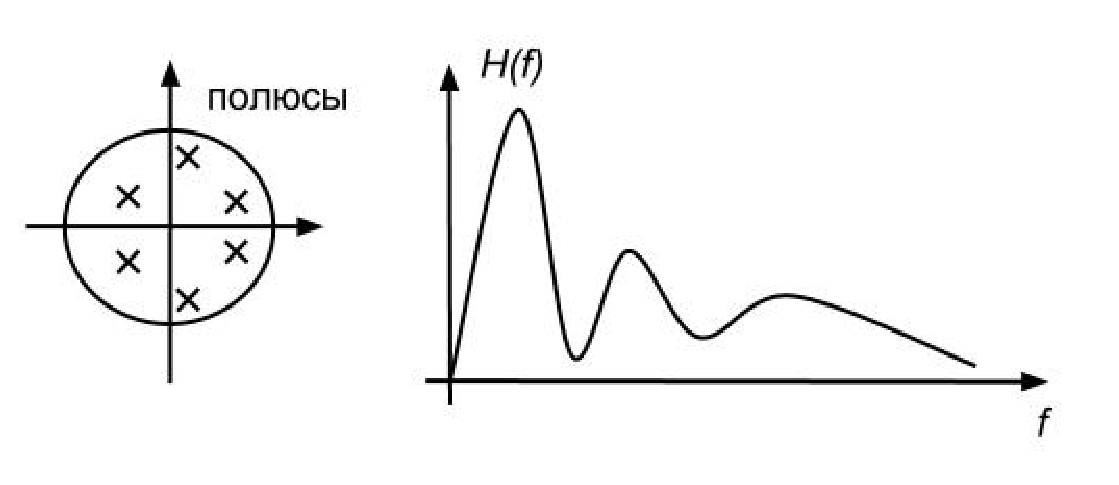
\includegraphics[width=1\linewidth]{lpc_poles.eps}}
%	\caption{Полюса и АЧХ линейного предсказателя}
%	\label{pic:lpc_poles}
%\end{figure}

{\bf{\textit{Вычисление коэффициентов АР-модели}}}

Наилучшие оценки коэффициентов ${a_k}$ могут быть получены минимизацией среднеквадратичной ошибки уравнения \cite{saeed_book} (\ref{eq:lpc_error}):
\begin{eqnarray}
	\label{eq:lpc_rms}
		E[e^2(m)]	& = & E[(x(m) - \sum \limits_{k=1}^P a_k x(m-k))^2] =\nonumber \\
				& = & E[x^2(m)] - \nonumber \\
				& &  - 2\sum \limits_{k=1}^P a_k E[x(m-k)x(m)] + \nonumber \\
				& &  + \sum \limits_{k=1}^P a_k \sum \limits_{j=1}^P a_j E[x(m-k)x(m-j)] = \nonumber \\
				& = & r_{xx}(0) - 2{\bf r}^T_{xx}{\bf a} + {\bf a}^T {\bf R_{xx}a},
\end{eqnarray}
где ${{\bf R_{xx}} = E[{\bf xx}^T]}$ - это автокорреляционная матрица входного вектора \\
${{\bf x}^T=[x(m-1),x(m-2),...,x(m-P)]}$,
${{\bf r}_{xx}=E[x(m){\bf x}]}$ - автокорреляционный вектор, а ${a^T=[a_1,a_2,...,a_P]}$ -  вектор коэффициентов предсказателя.
Процедура минимизации среднеквадратичной ошибки из уравнения (\ref{eq:lpc_rms}) может быть записано как:
\begin{equation}
	\label{eq:lpc_rms2}
	{\bf a=R^{-1}_{xx}r_{xx}},
\end{equation}
где матрица ${\bf R_{xx}}$ является теплицевой и эрмитовой, поскольку  ${r_{xx}(-k) = r_{xx}(k)}$.

Данная процедура является реализацией алгоритма Юла-Уокера. В этом алгоритме предполагается, что истинные значения
АКП ${r_{xx}(k)}$ известны. На практике значения АКП не известны и их приходится заменять оценкой ${\hat{r}_{xx}(k)}$, что может
при несмещенных оценках ${\hat{r}_{xx}(k)}$ привести к не положительно определенной матрице ${\bf {R_{xx}}}$, а значит
к неустойчивой \mbox{АР-модели} \cite{bolshakov-book}.

В случае вычисления параметров АР-модели путем решения уравнений Юла-Уокера, нахождение полюсов
внутри единичной окружности не очевидно. В \cite{shahtarin-spectrum-book} показано, что если
автокорреляционная матрица  ${{\bf R_{xx}}}$ является определенной положительно, то и решение
линейных уравнений Юла-Уокера порождает устойчивый только полюсный фильтр.

При больших объемах выборки входных данных, алгоритм Юла-Уокера дает вполне приемлемые результаты, в то время
как при малых выборках оценки параметров дают СПМ с низкой разрешающей способностью \cite{marpl_book, bolshakov-book}.

Можно использовать альтернативную запись.  Для сигнала длинной в ${N}$ отсчетов можно записать ${N}$ - уравнений:
\begin{equation}
	\label{eq:lpc_rms3}
	{\bf e=x-Xa}.
\end{equation}
Выражение (\ref{eq:lpc_rms3}) можно переписать в виде:
\begin{equation}
	\label{eq:lpc_rms4}
	{\bf e^T e = xx^T - 2x^T Xa + a^T X^T Xa}.
\end{equation}

Взяв производную по вектору ${{\bf a}}$, можно получить параметры предсказателя:
\begin{equation}
	\label{eq:lpc_rms5}
	\frac{\partial {\bf e^T e}}{\partial {\bf a}} = {\bf - 2x^T X + a^T X^T X} = 0.
\end{equation}
Из (\ref{eq:lpc_rms5}), коэффициенты для минимальной среднеквадратичной ошибки равны:
\begin{equation}
	\label{eq:lpc_rms6}
	{\bf a= (X^T X)^{-1} (X^T x)}.
\end{equation}

Сравнивая уравнение (\ref{eq:lpc_rms2}) и уравнение (\ref{eq:lpc_rms6}), видно, что в (\ref{eq:lpc_rms2})
автокорреляционная матрица и вектор заменены оценками:
\begin{equation}
	\label{eq:lpc_rxx_estimation}
	\hat{r}_{xx}(m) = \frac{1}{N} \sum \limits_{k=0}^{N-1} x(k)x(k-m).
\end{equation}

Для решения уравнения Юла-Уокера можно применить метод Гаусса, а также его модификации: LU-разложение,
разложение Холецкого, UD-разложение. Данные методы требуют выполнения вычислительных операций, пропорционально ${P^3}$.
Но, так как ${\bf{R^{-1}_{xx}}}$ в (\ref{eq:lpc_rms2}) является теплицевой и эрмитовой, можно использовать эффективные методы работы
с теплицевыми матрицами, которые значительно лучше упомянутых выше. 
Например, можно воспользоваться, быстрым алгоритмом Левинсона-Дарби.
Быстрым алгоритмам над теплицевыми матрицами посвящена книга \cite{bleyhut_book}.

АР-метод оценки СПМ часто используется для того, чтобы выявить в данных наличие синусоидальных
компонент. Мощность, соответствующую  таким компонентам в АР оценке СПМ, можно вычислить, интегрируя
площадь под кривой этой оценки. Однако это связано с большими вычислительными затратами, поэтому
гораздо более эффективным является использования в качестве показателя мощности синусоидальных
компонент высоты соответствующих им спектральных пиков \cite{marpl_book}.  

%%%%%%%%%%%%%%%%%%%%%%%%%%%%%%%%%%%%%%%%%%%%%%%%%%%%%%%%%%%%%%
{\bf{\textit{АР-модель второго порядка. Оценка частоты основного тона на основе АР-модели}}}

АР-модель второго порядка применяется для определения частоты основного тона. Для поиска единственного
тона необходимо найти 2 полюса. Тогда выражение (\ref{eq:lpc_rms2}) может быть записано как:
\begin{equation}
	\label{eq:lpc_a_estimation}
	\left[ \begin{array}{c}
		\hat{a}_1 \\
		\hat{a}_2
	\end{array} \right]
	=
		\left[ \begin{array}{cc}
			r_{xx}(0)  + \sigma_n^2 & r_{xx}(1)\\
			r_{xx}^*(1) & r_{xx}(0) + \sigma_n^2 
		\end{array} \right]^{-1}
		\left[ \begin{array}{c}
			r_{xx}(1) \\
			r_{xx}(2)
		\end{array} \right]
	= \bf{R_{xx}^{-1}r_{xx}},
\end{equation}
где ${\hat{a}_1, \hat{a}_2}$, - МНК оценки коэффициентов АР-модели, ${r_{xx}(m)}$ - АКФ принимаемого сигнала.
Для оценки АКФ  можно использовать выражение (\ref{eq:lpc_rxx_estimation}).

Передаточная функция АР-модели второго порядка ${H(z)}$:
\begin{equation}
	\label{eq:lpc_spectral_func}
	H(z) = \frac{1}{1 - a_1 z^{-1} - a_2 z^{-2}}.
\end{equation}

Характеристическое уравнение
\begin{equation}
	\label{eq:lpc_characteristic}
	z^2 - a_1 z - a_2 = 0.
\end{equation}
имеет полюсы
\begin{equation}
	\label{eq:lpc_poles_2}
	z_{1,2} =\frac{a_1 \pm \sqrt{a_1^2 + 4 a_2}}{2}.
\end{equation}

Для определения резонансной частоты ${H(z)}$ можно воспользоваться формулой (\ref{eq:lpc_poles_freq}).
Для принятия решения о наличии гармонического сигнала анализируют значение квадрата модуля частотной
характеристики АР-модели в точке резонанса:
\begin{equation}
	\label{eq:lpc_power_cos}
	\left| H(z) \right|^2 = \frac{1}{\left| 1 - a_1 e^{-j \omega_0} - a_2 e^{-2 \omega_0} \right|^2}.
\end{equation}

Если это значение превышает некоторый заранее выбранный порог, то принимается решение о наличии гармонического
сигнала с частотой ${\omega_0}$. 

%%%%%%%%%%%%%%%%%%%%%%%%%%%%%%%%%%%%%%%%%%%%%%%%%%%%%%%%%%%%%%
\section{Использование АР-модели для оценки параметров ШПС}

При работе с ПСП следует учитывать, что после демодуляции входного сигнала выровненной ПСП в сигнале восстанавливается одна гармоническая
компонента на промежуточной частоте, что дает возможность использовать АР-модель второго порядка.
Повторная модуляция сигнала с ПСП по любой фазе, отличной от искомой, не будет восстанавливать гармонический сигнал.
Спектр смеси гармонического сигнала, повторно модулированного ПСП с невыровненной фазой, будет похож на спектр исходной смеси – отображен
на Рис. \ref{pic:lpc_psd_1} штриховой пунктирной линией. И только повторная модуляция с выровненной фазой ПСП даст спектр
изображенный светлой сплошной линией на Рис. \ref{pic:lpc_psd_1}.
\begin{figure}[h]
	\center\scalebox{1}{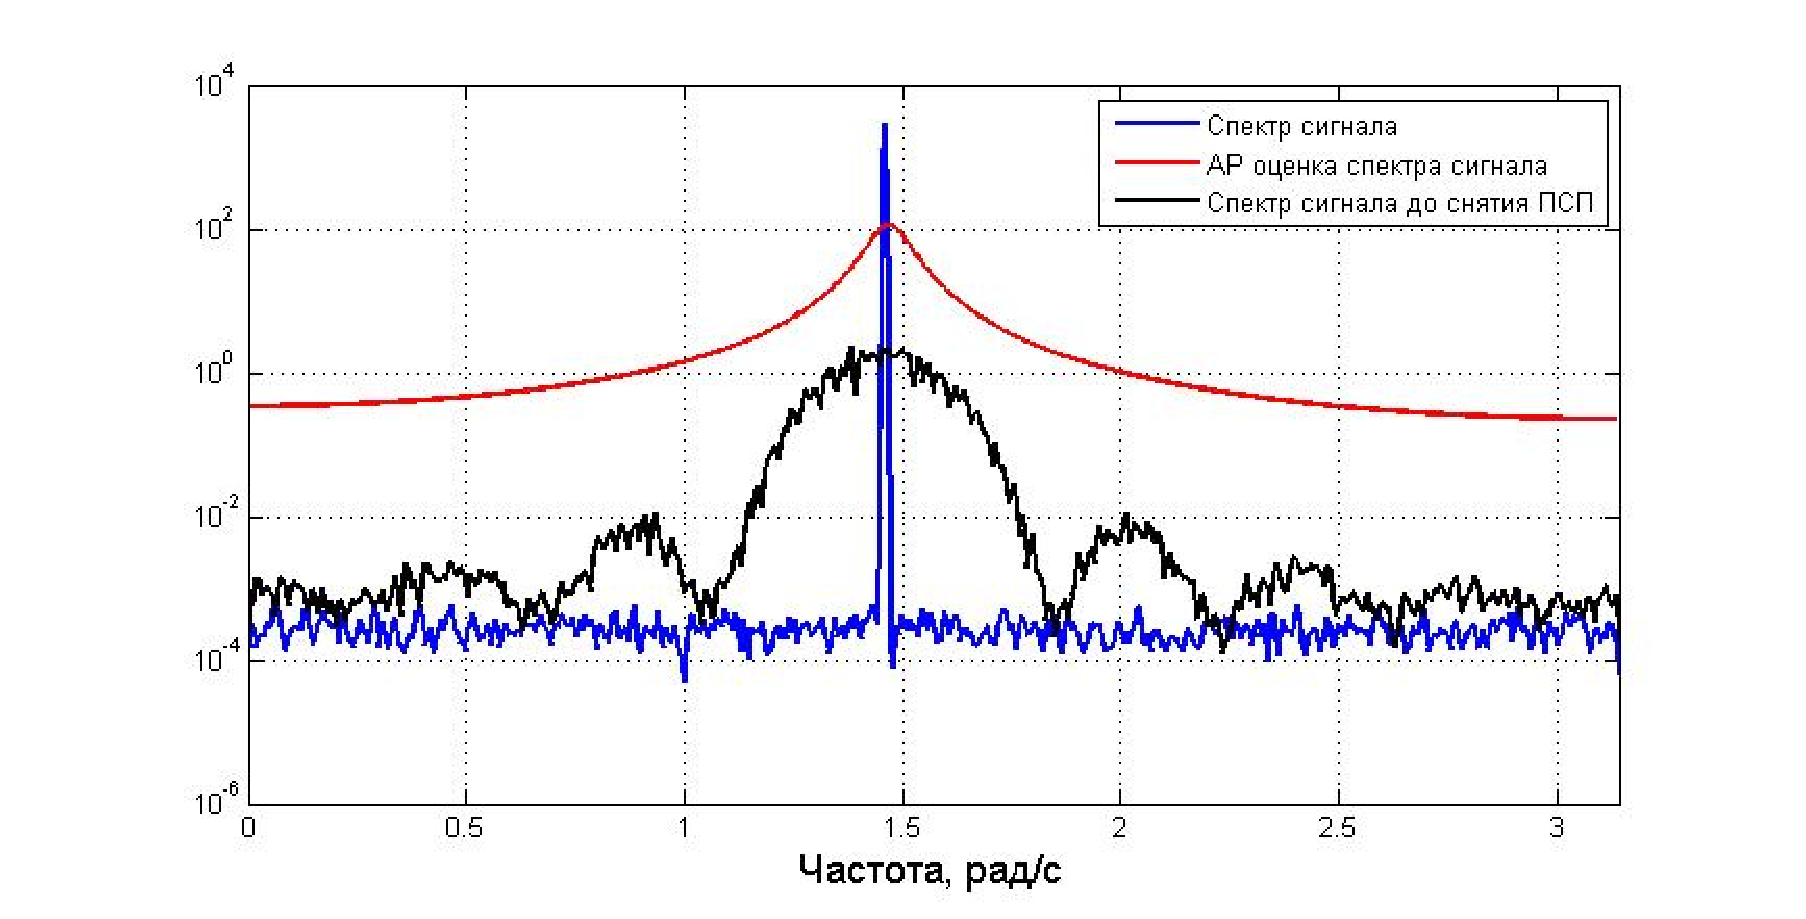
\includegraphics[width=1\linewidth]{lpc_1sat.eps}}
	\caption{Оценка СПМ сигнала, модулированного ПСП}
	\label{pic:lpc_psd_1}
\end{figure}

На \ref{pic:lpc_basic1} входная смесь повторно модулируется ПСП с известной фазой.
\begin{figure}[h]
	\center\scalebox{0.8}{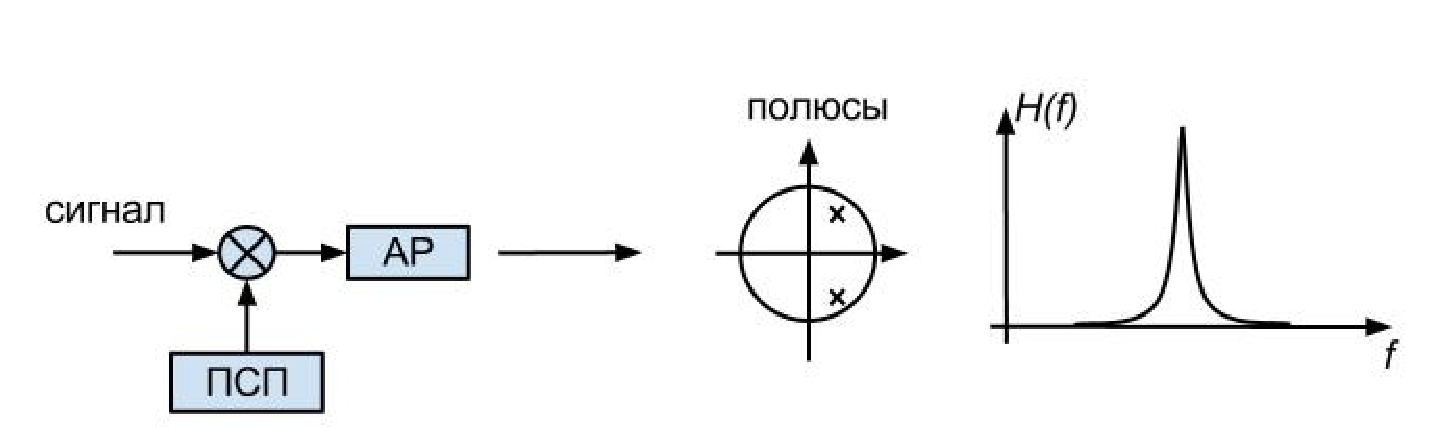
\includegraphics[width=1\linewidth]{lpc_basic.eps}}
	\caption{Общая схема применения АР-модели для детектирования ШПС сигнала}
	\label{pic:lpc_basic1}
\end{figure}

На выходе алгоритма будет СПМ, а пик будет соответствовать энергии на определенной частоте.

%На Рис.  \ref{pic:lpc_poles_gps} красным изображена энергия гармонического колебания с большой мощностью, а зеленым изображен цветной шум.
%\begin{figure}[h]
%	\center\scalebox{1}{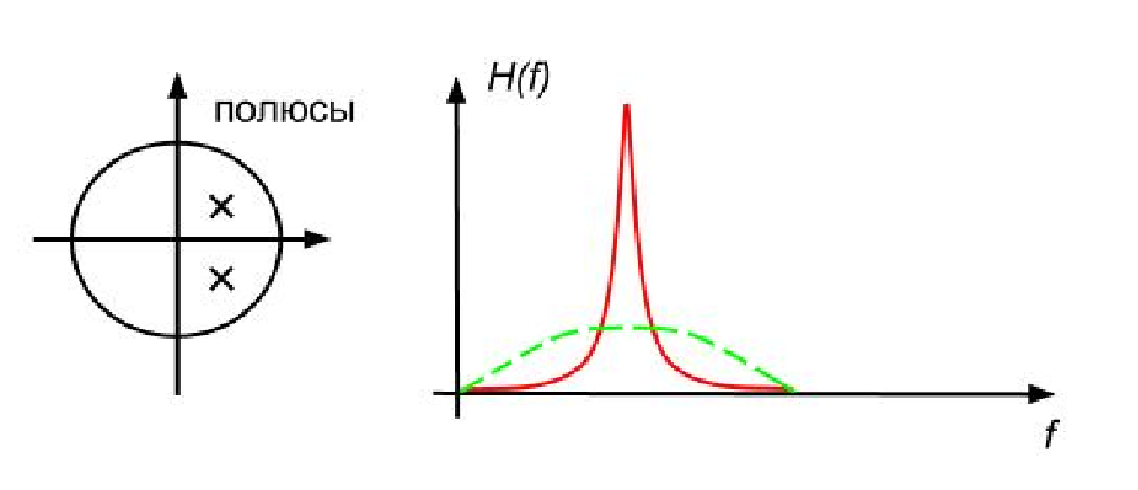
\includegraphics[width=1\linewidth]{lpc_poles_gps.eps}}
%	\caption{Полюс и АЧХ линейного предсказателя}
%	\label{pic:lpc_poles_gps}
%\end{figure}

Так же необходимо отметить, что фаза ПСП в момент начала приема сигнала не известна.
Для оценки частоты сигнала необходимо для каждой фазы ПСП вычислить квадрат частотного
отклика.

Описанный алгоритм состоит из следующих шагов (${\tau \in [0, \tau_{max}]}$):
\begin{itemize}[align=left,style=nextline,leftmargin=*,labelsep=\parindent,font=\normalfont]
\item[Шаг 1.] Вычисляются оценки АКФ в трех точках (для аргументов АКФ=0,1,2)
	для фазы ПСП ${\tau}$, по формуле (\ref{eq:lpc_rxx_estimation}). 
\item[Шаг 2.] Определяются коэффициенты АР-модели ${\hat{a_1}, \hat{a_2}}$, 
	по формуле (\ref{eq:lpc_a_estimation}). 
	Вычисляется резонансная частота ${\omega_0}$ по формуле (\ref{eq:lpc_poles_freq})
	и определяется квадрат модуля частотного отклика АР-модели для этой частоты по выражению (\ref{eq:lpc_power_cos}). 
\item[Шаг 3.] Полученное значение квадрата частотного отклика сравнивается с заранее выбранным порогом детектора. 
	\subitem{\bf{Если}}  значение оказалось больше порогового, {\bf{то}} 
		принимается решение о наличии сигнала, а в качестве оценки
		частоты принимается значение ${\omega_0}$ соответствующее смещению ПСП равному ${\tau}$. 
	\subitem{\bf{Иначе если}} ${\tau}$ меньше длины ПСП ${\tau = \tau + 1}$, переход к шагу 1.
	\subitem{\bf{Иначе}} 
		Принимается решение об отсутствии гармонического сигнала.
\end{itemize}

Квадраты модулей частотного отклика для всех возможных значений фазы в пределах одной ПСП представлены на Рис. \ref{pic:lpc_1sat_energy}.
\begin{figure}[h]
	\center\scalebox{1}{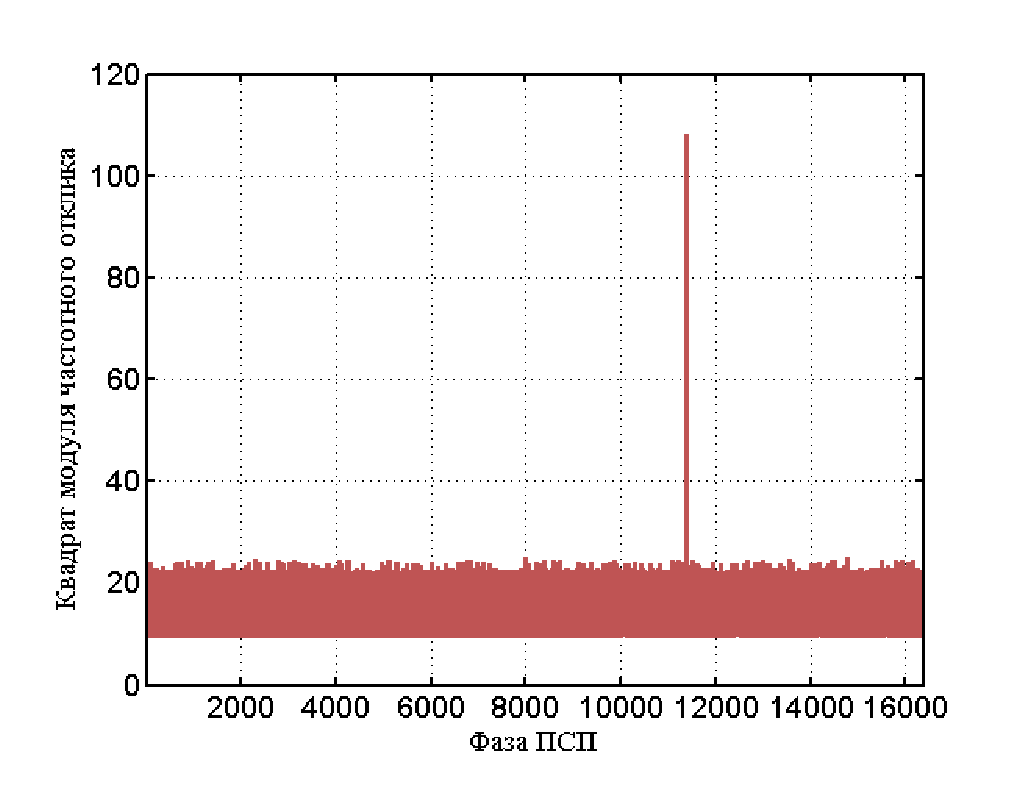
\includegraphics[width=1\linewidth]{lpc_1sat_energy.eps}}
	\caption{Квадраты частотного отклика для всех возможных фаз ПСП}
	\label{pic:lpc_1sat_energy}
\end{figure}

%%%%%%%%%%%%
% My algo

Алгоритм оценки параметров на основе АР-модели требует значительных вычислительных затрат, так как требуется проводить
повторную модуляцию и оценку параметров \mbox{АР-модели} по каждому смещению ПСП.

Для перебора фаз ПСП воспользуемся БПФ, в результате получим значения оценки АКФ для каждой фазы ПСП \cite{my_lpc_for_1, my_lpc_for_1_controllers}.
Схема алгоритма представлена на Рис. \ref{pic:lpc_basic2}. 

\begin{figure}[h]
	\center\scalebox{0.9}{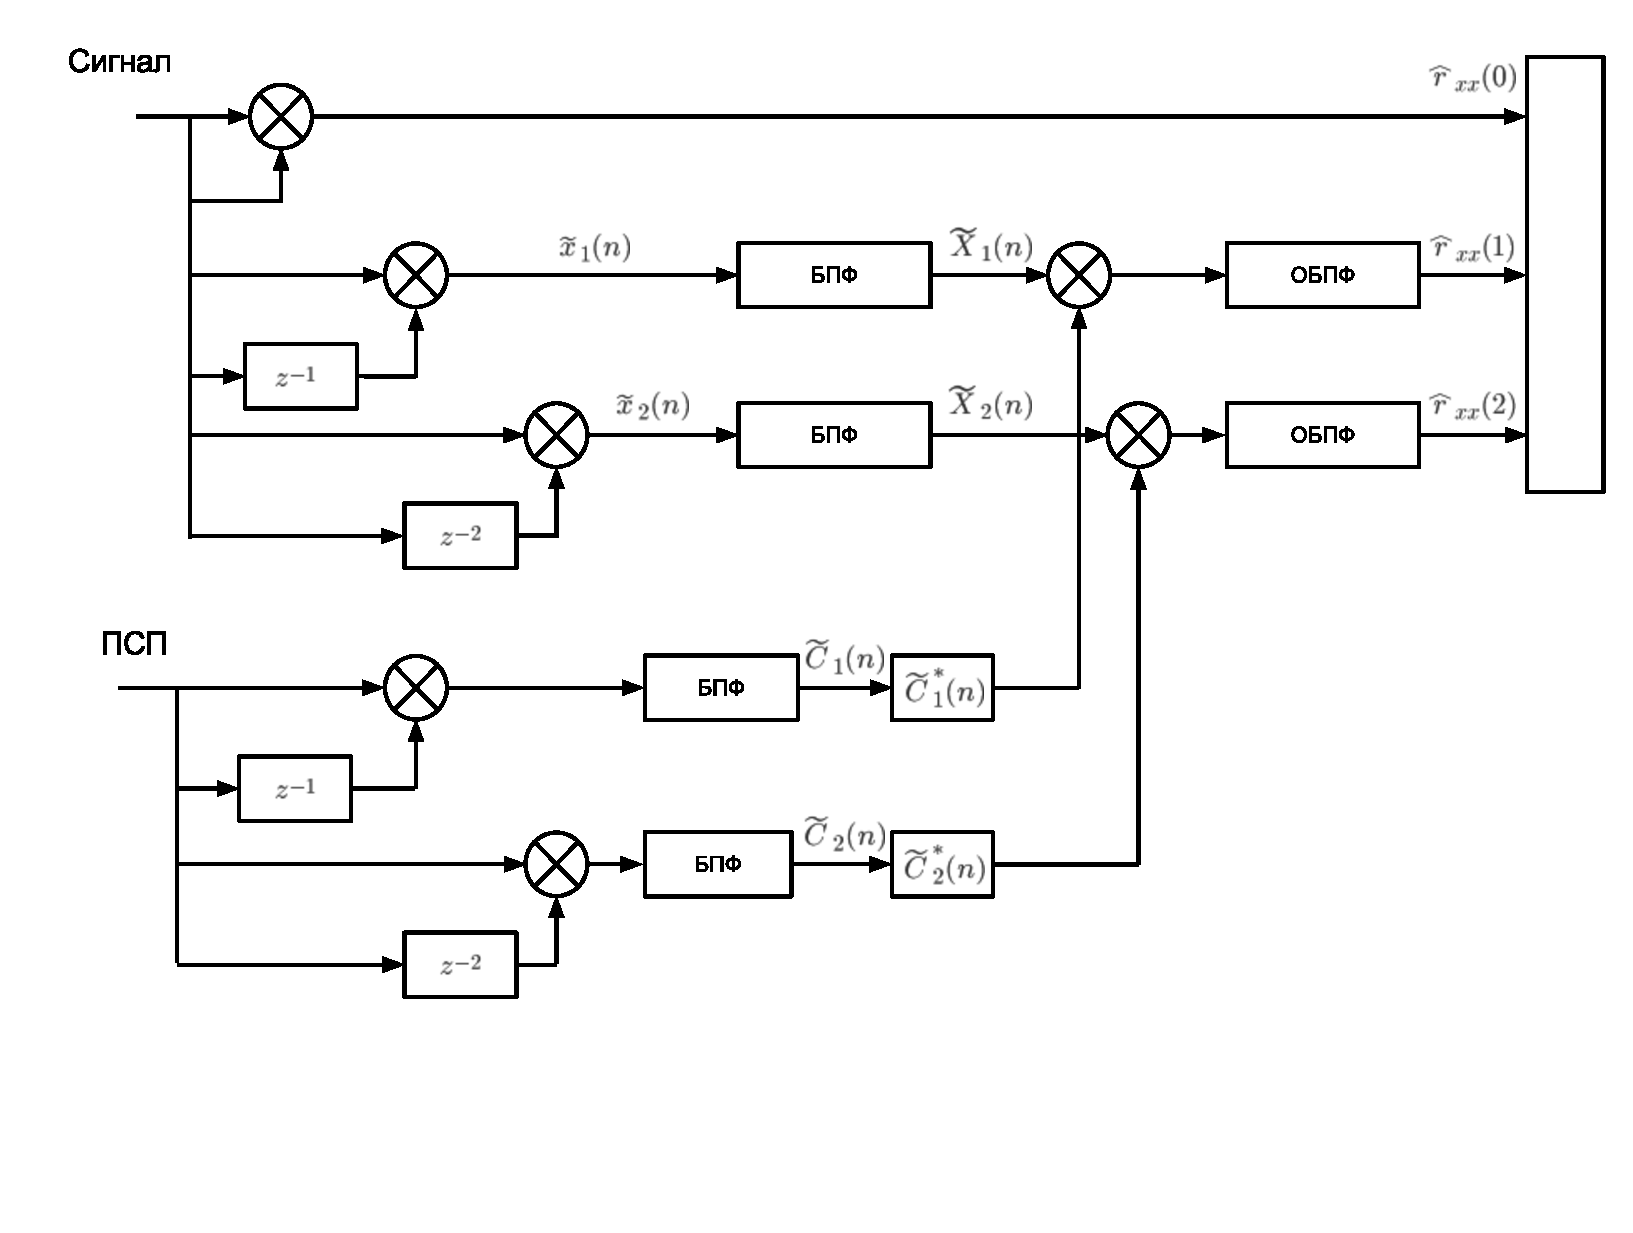
\includegraphics[width=1\linewidth]{lpc_fft.eps}}
	\caption{Схема применения АР-модели для детектирования ШПС сигнала с оптимизацией}
	\label{pic:lpc_basic2}
\end{figure}

Оценка АКФ ${\hat{r}_{xx}(0)}$ не зависит от выбранной фазы ПСП, поэтому она вычисляется один
раз для всех фаз ПСП. Далее формируется массив произведений входной смеси на
свою задержанную копию ${\tilde{x}_1(m)=x(m)x(m-1)}$. Полученная последовательность  
${\tilde{x}_1(m)}$ поступает на вход алгоритма БПФ, в результате получаем массив ${\tilde{X}_1(n)}$.
Аналогично формируется массив  ${\tilde{X}_2(m)}$ для
задержки входной смеси равной двум. Таким же способом обрабатываются локально
сгенерированные ПСП и формируются два массива ${\tilde{G}_1(m)}$ и ${\tilde{G}_2(m)}$.
Далее массивы ${\tilde{X}_1(m)}$ и ${\tilde{X}_1(m)}$ поэлементно перемножаются
на массивы ${\tilde{G}_1^*(n)}$ и ${\tilde{G}_2^*(m)}$, комплексно сопряженные к массивам ${\tilde{G}_1(m)}$ и ${\tilde{G}_2(m)}$.
Результаты этих перемножений поступают на вход алгоритма обратного
БПФ (ОБПФ). Полученные после ОБПФ два массива содержат оценки автокорреляционной функции для ${N}$ 
фаз, где  ${N}$ - размер данных на входе алгоритма БПФ.

Таким образом, предлагаемый алгоритм состоит из следующих шагов:

\begin{itemize}[align=left,style=nextline,leftmargin=*,labelsep=\parindent,font=\normalfont]
\item[Шаг 1.] Вычисляются оценки  АКФ в трех первых точках (для аргументов АКФ=0,1,2)
	с использованием алгоритма БПФ для всех возможных смещений ПСП. 
\item[Шаг 2.] Для каждого смещения ПСП: 
	Определяются коэффициенты АР-модели ${\hat{a_1}, \hat{a_2}}$, 
	по формуле (\ref{eq:lpc_a_estimation}). 
	Вычисляется резонансная частота ${\omega_0}$
	и определяется квадрат модуля частотного отклика АР-модели для этой частоты. 
\item[Шаг 3.] Выбирается смещение ПСП для которого значение квадрата модуля частотного отклика было максимальным. Полученное значение сравнивается с заранее выбранным порогом детектора. 
	\subitem{\bf{Если}}  значение оказалось больше порогового, {\bf{то}} 
		принимается решение о наличии сигнала, а в качестве оценки
		частоты принимается значение ${\omega_0}$ соответствующее выбранному смещению ПСП. 
	\subitem{\bf{Иначе}} 
		Принимается решение об отсутствии гармонического сигнала.
\end{itemize}

Количество операций для оценки параметров от одного источника на фоне АБГШ:
\begin{equation}
	%\label{}
	OP_{AR\_FOR\_1} = 24NlogN + 63N,
\end{equation}
где ${N}$ - длинна входной последовательности.

%%%%%%%%%%%%%%%%%%%%%%%%%%%%%%%%%%%%%%%%%%%%%%%%%%%%%%%%%%%%%%
{\bf{\textit{Влияние теплового шума на точность оценки частоты с помощью АР-модели}}}
Серьезным фактором, ограничивающим применение АР-модели при оценке параметров гармонического сигнала является
его чувствительность к шуму. В особенности к окрашенному шуму.

На Рис. \ref{pic:lpc_psd_2} представлена оценка СПМ для ШПС при наличии интерференции.
\begin{figure}[h]
	\center\scalebox{1}{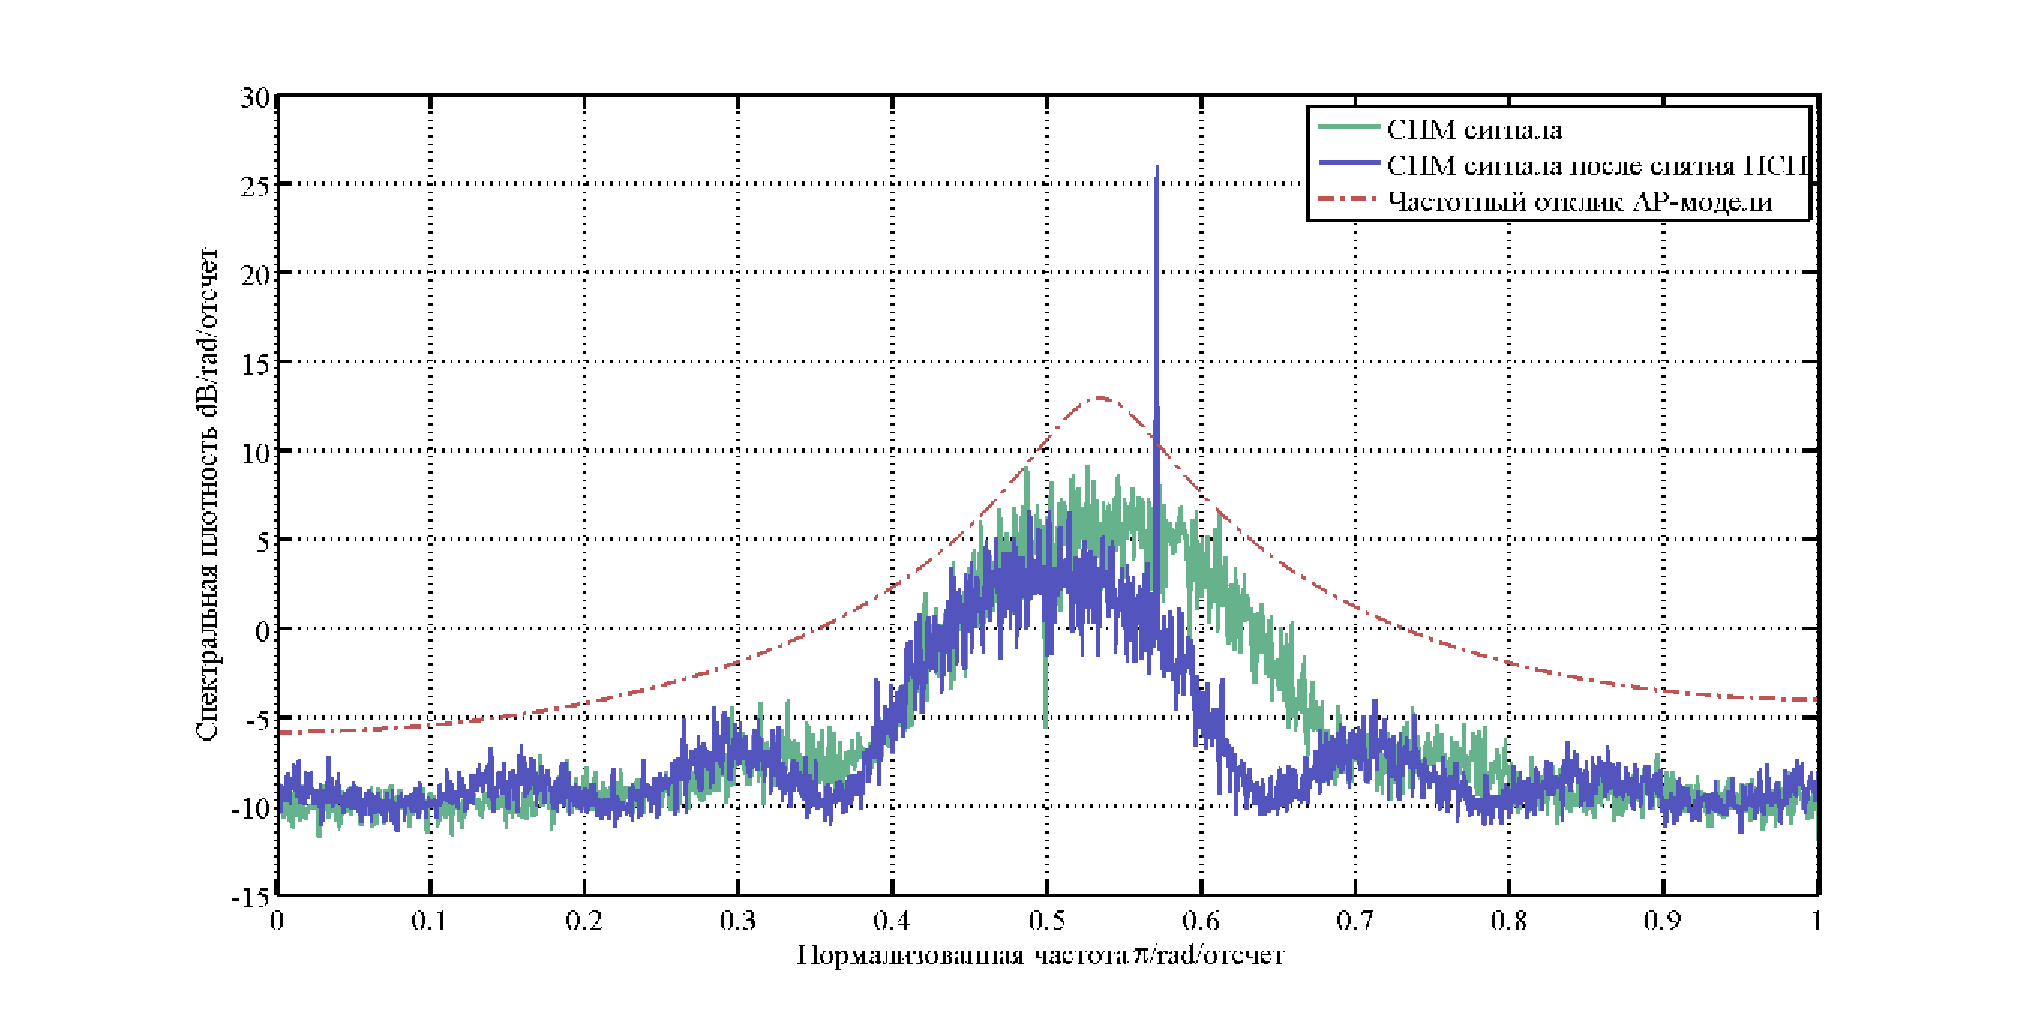
\includegraphics[width=1\linewidth]{lpc_2sat_psd.eps}}
	\caption{Оценка СПМ сигнала, модулированного ПСП при наличии интерференционной помехи}
	\label{pic:lpc_psd_2}
\end{figure}

Наличие в данных интерференционной составляющей сильно смещает оценку. Ввиду данного факта, предлагаемый алгоритм в исходном виде
не может быть применен в реальных системах, так как реальные системы обладают множеством каналов, разделенных кодом ПСП. Поэтому предложенный алгоритм,
основанный на \mbox{АР-методе}, нуждается в ряде усовершенствований чтобы удовлетворять критериям реальных систем.

%%%%%%%%%%%%%%%%%%%%%%%%%%%%%%%%%%%%%%%%%%%%%%%%%%%%%%%%%%%%%%
\section{Сравнение точности оценки с границей Крамера-Рао}
График вероятности оценки частоты в допустимом диапазоне входной расстройки модуля фазовой автоподстройки частоты (ФАПЧ) представлен на Рис.
\ref{pic:lpc_for_1_probability}. Моделирование проводилось с аддитивным шумом, заданным в полосе от 0 Гц до
половины частоты дискретизации для одного источника. В данном случае значение частоты дискретизации равно 16.368 МГц.
\begin{figure}[H]
\center\scalebox{1}{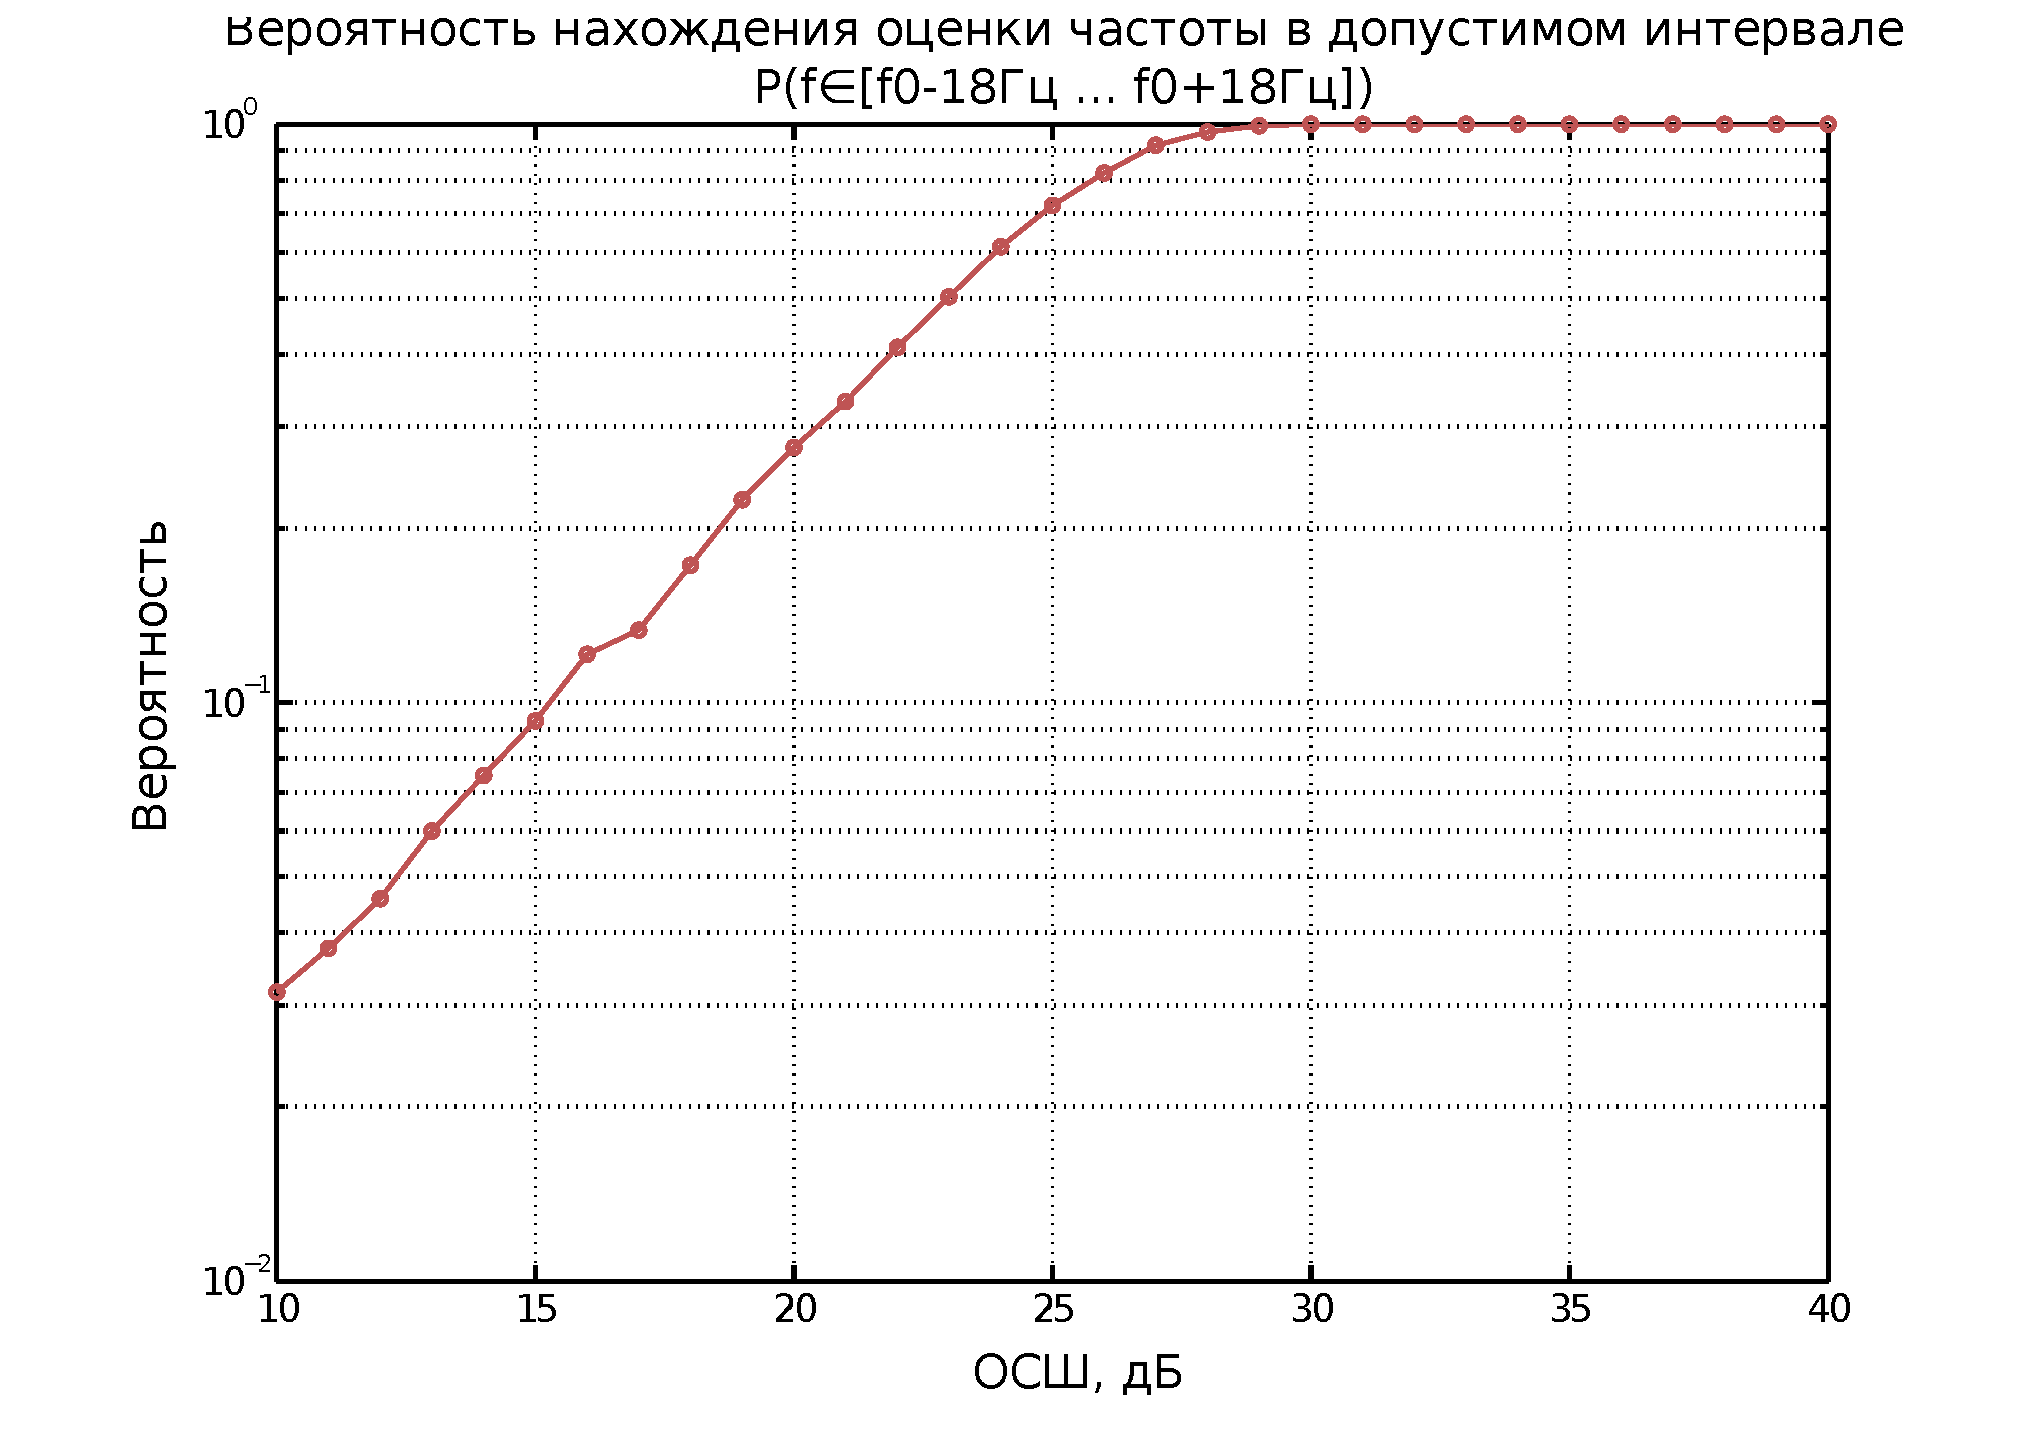
\includegraphics[width=1\linewidth]{lpc_for_1_probability.eps}}
	\caption{Вероятность нахождения оценки частоты в интервале, удовлетворяющем допустимой входной расстройке ФАПЧ}
	\label{pic:lpc_for_1_probability}
\end{figure}

Для оценки точности можно сравнить предлагаемый алгоритм с границей Крамера-Рао (КР). Неравенство Крамера-Рао дает базу оценки, так
как представляет минимальную дисперсию оцениваемой величины среди всех классов оценщиков.
\begin{figure}[H]
\center\scalebox{1}{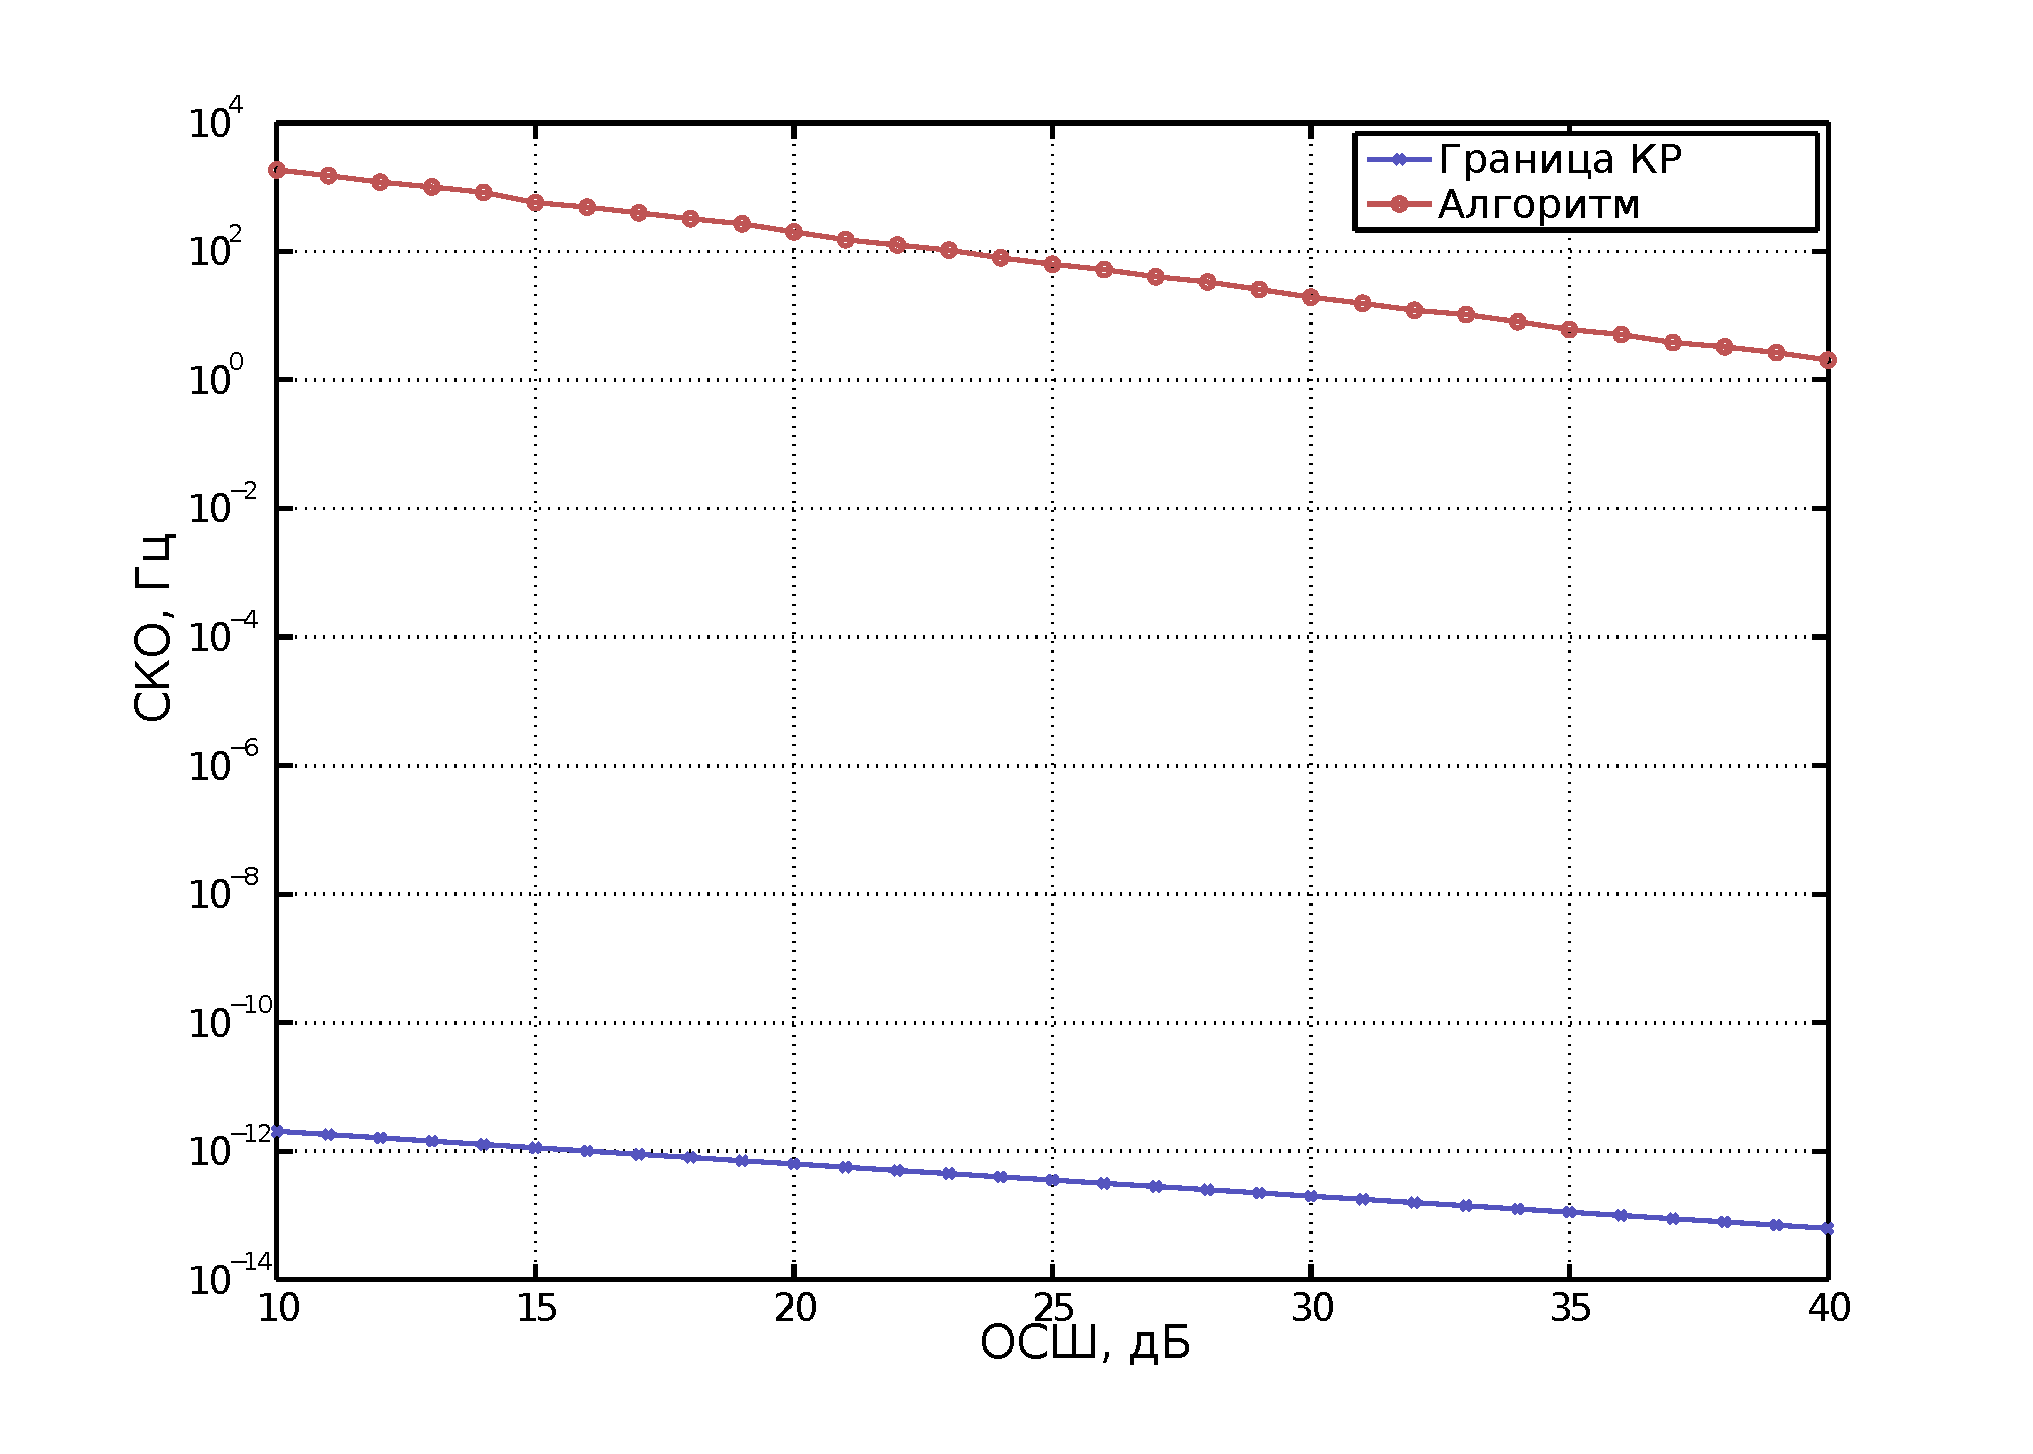
\includegraphics[width=1\linewidth]{crlb_vs_1sat_algo.eps}}
	\caption{СКО оценки частоты}
	\label{pic:crlb_vs_1sat_algo}
\end{figure}

Как видно из \mbox{Рис. \ref{pic:crlb_vs_1sat_algo}} алгоритм оценки информационных параметров для одного источника сигнала в CDMA-системах на фоне АБГШ позволяет снизить вычислительные
затраты в 1.5 раза в сравнении с типовым подходом при этом точность оценки, при отсутствии МКИ, не превосходит нескольких десятков герц для сигналов
с ОСШ более 25 дБ.


%%%%%%%%%%%%%%%%%%%%%%%%%%%%%%%%%%%%%%%%%%%%%%%%%%%%%%%%%%%%%%
\section{Выводы по Главе 1}

\begin{enumerate}
\item Задачу оценки информационных параметров ШПС СНС Navstar GPS с кодовым разделением каналов (CDMA) можно решить с помощью алгоритма на основе АР-модели,
	отличительной особенностью которого является сведение перебора в двухмерной области неопределенности к перебору только по фазе ПСП и оценке
	резонансной частоты, повторно модулированного ПСП сигнала, при помощи АР-модели.

\item К достоинству данного алгоритма можно отнести то, что он позволяет снизить вычислительные затраты в 1.5 раза в сравнении с типовым подходом.
	Вычислительная сложность - общее количество умножений для оценки информационных параметров для одного источника сигнала в CDMA-системах на фоне АБГШ:
	${OP_{AR\_FOR\_1} = 24NlogN + 63N}$.


\item В предложенный алгоритм включена операция оценки оценки полюсов АР-модели, которая требует вычислений с плавающей точкой, а значит программно-аппаратная
	платформа должна иметь модуль для вычислений с плавающей точкой (в иностранной литературе floating point unit - FPU).

\item Результаты имитационного моделирования показали высокую чувствительность алгоритма к МКИ, что приводит к значительному смещению получаемых оценок
	частоты и мощности гармонического сигнала. Поэтому алгоритм на основе АР-модели требует усовершенствования.

\item В результате имитационного моделирование также была получено значение СКО точности оценки частоты. СКО оценки не превосходит нескольких десятков герц для сигналов
	с ОСШ более \mbox{25 дБ}.

%%%%%
%\item Разработан алгоритм на основе параметрического метода оценки информационных для одного источника с CDMA-сигналом на фоне аддитивного белого гауссового шума при отстутствии МКИ.
%	Получены значение вычислительной сложности и точности оценки частоты. Алгоритм на основе параметрического метода оценки частоты позволяет снизить вычислительные
%	затраты в 1.5 раза в сравнении с типовым подходом при этом точность оценки, при отсутствии МКИ, не превосходит нескольких десятков герц для сигналов
%	с ОСШ более 25 дБ.
%\item Вычислительная сложность - общее количество умножений для оценки частоты при помощи алгоритма оценки информационных параметров ШПС на фоне АБГШ c использованием \mbox{АР-модели}:
%	${OP_{AR\_FOR\_1} = 24NlogN + 63N}$.
%\item Оценка полюсов АР-модели требует вычислений с плавающей точкой, а значит программно-аппаратная платформа должна иметь модуль для вычислений с плавающей точкой
%	(в иностранной литературе floating point unit - FPU).
%\item Высокая чувствительность к МКИ - наличие окрашенного  шума приводит к значительному смещению получаемых оценок частоты и мощности гармонического сигнала.
\end{enumerate}

%%%%%%%%%%%%%%%%%%%%%%%%%%%%%%%%%%
%В реальных СПИ сигнал на приемник поступает одновременно от нескольких источников, присутствует неопределенность по частоте, а также аддитивный белый шум (АБГШ).
%В приемнике после оцифровки сигнала получаем смесь:
%\begin{equation}
%	\label{eq:cdma_strip_eq}
%	x(m)=\sum_{k=1}^{N}\left( A_k g(m + \tau_k)\exp{\left[j \left( \tilde{\omega}_{k}m + \phi_k(m)\right)\right]} \right) + n(m),
%\end{equation}
%где  ${k}$ - относительный номер источника сигнала, ${N}$ - количество доступных источников сигнала, модулированных ПСП одного семейства,
%${m}$ - индекс соответствующий времени, ${\tilde{\omega}_{k}}$  – относительная частота, соответствующая ${\omega_0}$,
%${\tau_k}$ - задержка модулирующей ПСП в точке приема, ${\phi_k(m)}$ - случайная начальная фаза, ${n(m)}$ - аддитивный белый гауссов шум (АБГШ). 
%
%Следует отметить, что при оценке фазы сигнала с номером ${k}$  интерференцией являются сигналы:    .
%\begin{equation}
%	%\label{eq:cdma_interference}
%	\{n \ne k, n \in [1,N]\}
%\end{equation}

%\subsection{Постановка задачи оценки параметров сигнала с расширенным спектром}
%\paragraph{Основные свойства широкополосных сигналов}
%
%%%%%%%
%\paragraph{Классическая постановка задачи оценки параметра.}
%
%%%%%%%
%%%%%%%
%\paragraph{Алгоритмы оценки параметров широкополосного сигнала сигнала.}
%
%%%%%%%%%
%% Chaos 
%Оценка параметров СПИ с ШПС (в частности сигналов системы Navstar GPS) с помощью осциллятора Дуффинга
%достаточно новое направление в исследованиях по данной тематике. В данной области опубликовано несколько работ, в частности \cite{chaos_chen, chaos_cambridge, chaos_huang, chaos_song}.
%Так же является интересной более ранняя статья не рассматривающая GPS \cite{chaos_wang}.
%Осциллятор Дуффинга с гармоническим внешним воздействием может быть описан уравнением:
%\begin{center}
%\begin{equation}
%	\label{eq:duffing}
%	mx'' + cx' + k_{1}x + k_{2}x^3 = F_{0}\cos(\omega{t}),
%\end{equation}
%\end{center}
%где $m$ - масса, $c$ - коэффициент диссипации, $x$ - состояние осциллятора, $k_1$ и $k_2$ - линейный и нелинейный коэффициенты соответственно,
%$F_{0}\cos(\omega{t})$ - внешнее воздействие.
%
%Подробно уравнение \ref{eq:duffing} рассмотрено в \cite{chaos_neimark_landa}.
%Для использования осциллятора Дуффинга с целью оценки параметров ШПС была предложена усовершенствованная форма \cite{chaos_song, chaos_chen}:
%\begin{center}
%\begin{equation}
%	\label{eq:duffing_gps}
%	x'' +cx' - x^3 + x^5 = \gamma\cos(\omega{t}) + (\gamma_{x}\cos(\omega_{x}) + n(t))
%\end{equation}
%\end{center}
%
%Перепишем динамическую систему \ref{eq:duffing_gps} в виде:
%\begin{center}
%\begin{equation}
%	\label{eq:duffing_gps_2}
%	\left\{
%	\begin{aligned}
%		y(t) & = x'(t) \\
%		y'(t) & =  -cx' + x^3 - x^5 + \gamma\cos(\omega{t}) + (\gamma_{x}\cos(\omega_{x}) + n(t)),
%	\end{aligned}
%	\right.
%\end{equation}
%\end{center}
%где ${n(t)}$ - АБГШ.
%
%Пример фазового портрета при ${\omega=\omega_{x}}$ изображен на рисунке \ref{pic:duffing_sync},
%фазовый портрет хаоса расположен на рисунках \ref{pic:duffing_chaos1}, \ref{pic:duffing_chaos2}
%\begin{figure}[H]
%	\center\scalebox{0.5}{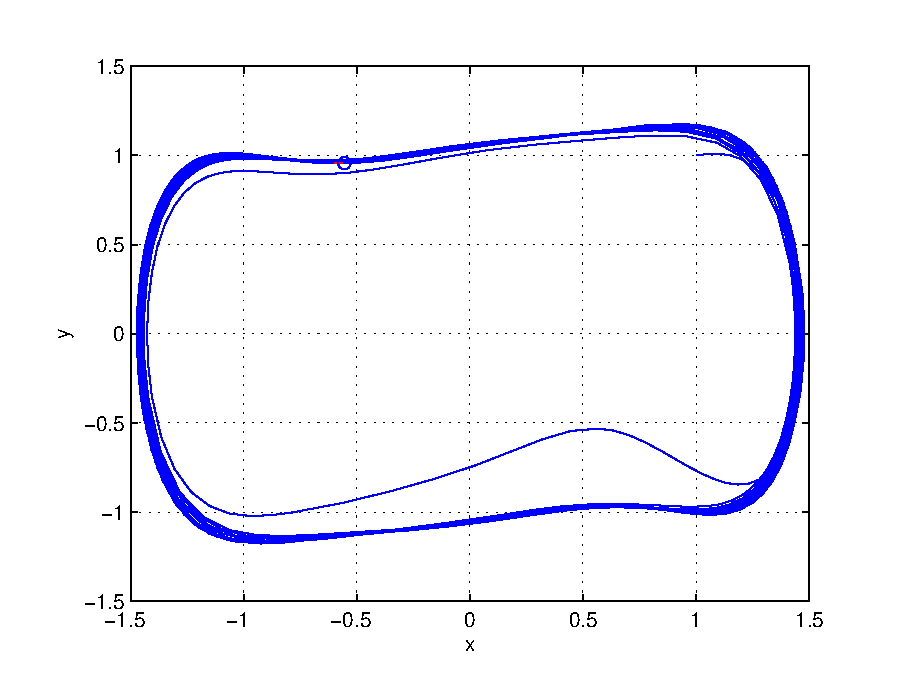
\includegraphics[width=1\linewidth]{duffing_sync.eps}}
%	\caption{Фазовый портрет при ${\omega =\omega_{x}}$}
%	\label{pic:duffing_sync}
%\end{figure}
%\begin{figure}[H]
%	\center\scalebox{0.5}{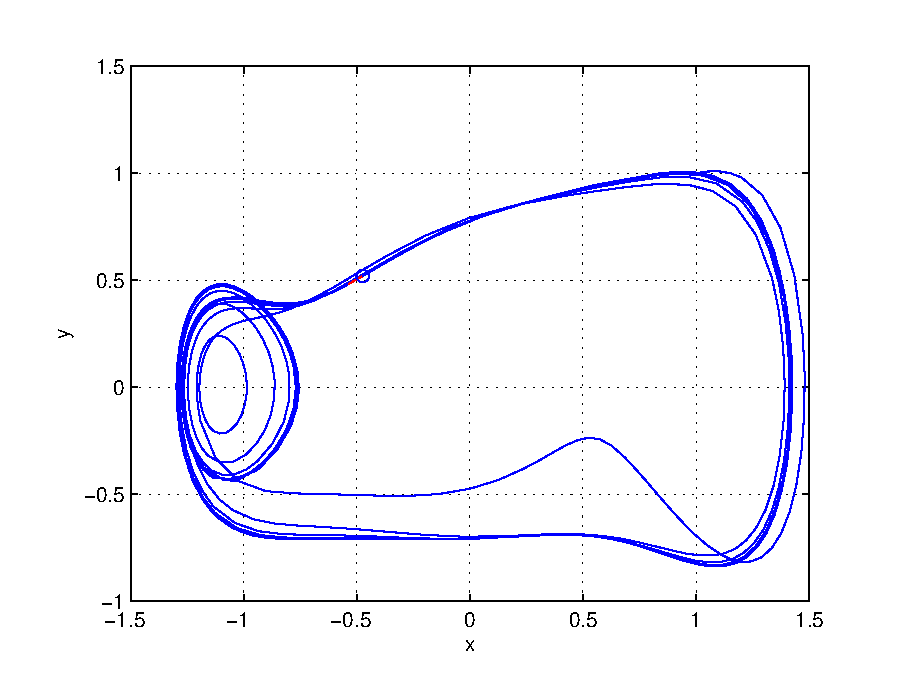
\includegraphics[width=1\linewidth]{duffing_chaos1.eps}}
%	\caption{Фазовый портрет при ${\omega < \omega_{x}}$}
%	\label{pic:duffing_chaos1}
%\end{figure}
%\begin{figure}[H]
%	\center\scalebox{0.5}{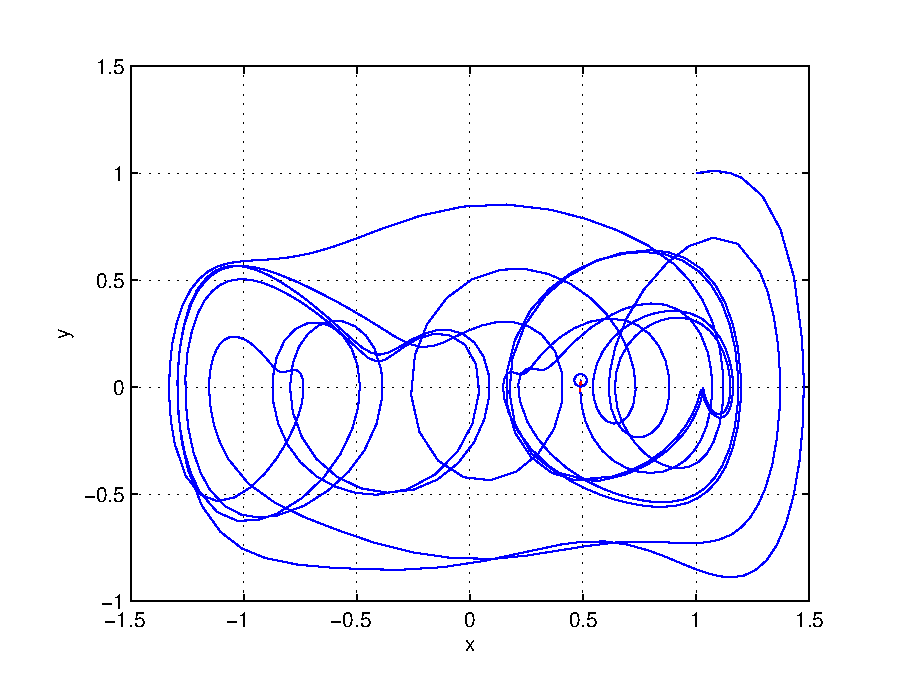
\includegraphics[width=1\linewidth]{duffing_chaos2.eps}}
%	\caption{Фазовый портрет при ${\omega > \omega_{x}}$}
%	\label{pic:duffing_chaos2}
%\end{figure}
%В качестве параметров уравнения применялись: $c = 0.5$, $\gamma=\gamma_{x}=0.36$, ${\omega=1}$
%
%Часто для вычисления характеристик хаотической динамики применяется показатель Ляпунова.
%Он показывает в каком состоянии находится система. Если система находится
%в стабильном состоянии линии фазовой траектории будут близко прилегать одна к другой, в противном
%случае система находится в состоянии хаоса. Детектор с применением показателя Ляпунова
%представлен на рисунке \ref{pic:chaos_lyapunov}.
%\begin{figure}[H]
%	\center\scalebox{0.7}{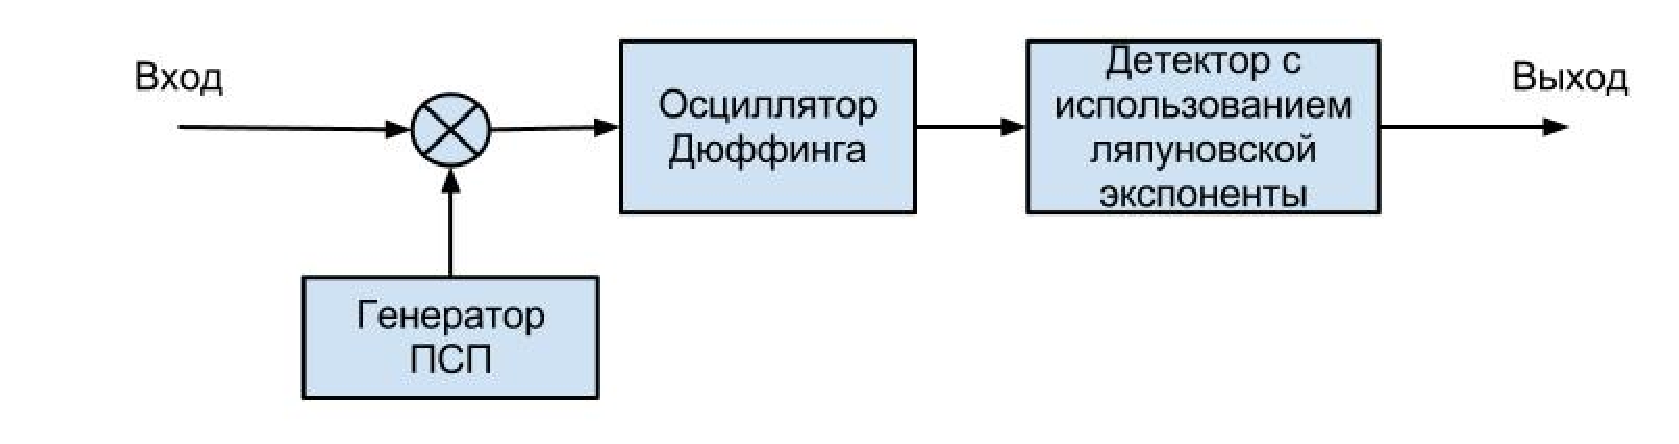
\includegraphics[width=1\linewidth]{Chaos_detector_Lyapunov.eps}}
%	\caption{Схема детектора основанного на показателе ляпунова для осциллятора Дуффинга}
%	\label{pic:chaos_lyapunov}
%\end{figure}
%
%В статье \cite{chaos_chen} предложен усовершенствованный метод, базирующийся на вычислении дисперсии
%фазовой траектории. Действительно, на рисунках \ref{pic:duffing_sync}, \ref{pic:duffing_chaos1},
%\ref{pic:duffing_chaos2} видно, что когда система находится в хаотическом состоянии значение
%дисперсии по координате ${x}$ больше, чем соответствующее значение в состоянии $\omega = \omega_{x}$.
%На основе этого была предложена усовершенствованная схема детектора сигнала - рисунок \ref{pic:chaos_energy_detector}
%\begin{figure}[H]
%	\center\scalebox{0.7}{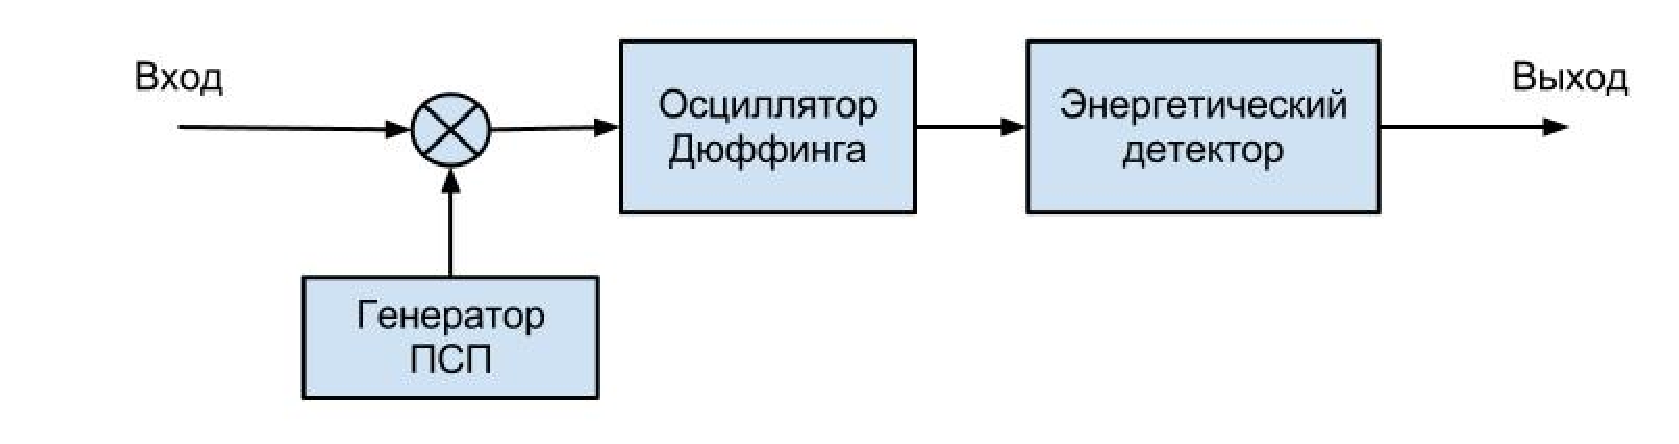
\includegraphics[width=1\linewidth]{chaos_detector.eps}}
%	\caption{Схема энергетического детектора для осциллятора Дуффинга}
%	\label{pic:chaos_energy_detector}
%\end{figure}
%
%%%%%%%%%
%% HOS 
%Математический аппарат статистик высоких порядков (СВП или HOS - Higher-order statistics)
%для исследования непричинных, причинных и нестабильных (систем с неминимальной фазой) и негауссовых сигналов впервые был предложен
%в \cite{hos_petropulu} в 1993 году.  Этот метод позволяет не только подавлять цветной Гауссов шум, но так же в некоторых случаях подавлять
%цветной не-Гауссов шум.
%
%В работе \cite{hos_zhao} был предложен метод детектирования ШПС с использованием СВП.
%
%%%%%%%%%
%% CHE 
%Интересная группа алгоритмов основывается на информационной избыточности ШПС, например \cite{phd_che}. В данной
%группе алгоритмов используется механизм появления нескольких точек на основном пике КФ, описанный в \cite{kaplan}. Пример
%изображен на рисунке \ref{pic:sec1_peak_tcd}.
%\begin{figure}[H]
%        \center\scalebox{1}{\includegraphics[width=1\linewidth]{corr_peak_tcd.eps}}
%        \caption{Идеальная КФ ШПС с отмеченными точками возможного обнаружения}
%        \label{pic:sec1_peak_tcd}
%\end{figure}
%На рисунке \ref{pic:sec1_peak_tcd} изображен пик КФ с несколькими точками. Две точки находятся выше порога ${\Pi=0.5}$.
%В работе \cite{phd_che} рассмотрено создание субоптимального обнаружителя на основе информационной избыточности ШПС.
%Получена целевая функция системы и намечены дальнейшие пути развития данного направления.
%
%%%%%%%%%
%% 2MAX 
%Так же одним из направлений исследований является разработка алгоритмов выбора порога без априорной информации о величине ОСШ. Например,
%в работах \cite{2max_ieee, 2max_article} представлен алгоритм нахождения пика (АНП) КФ (Peak-finding algorithm).
%
%Данный алгоритм можно разбить на несколько шагов:
%\begin{itemize}
%\item[Шаг 1] Подсчитать КФ, используя метод предложенный с использованием параллельного коррелятора. 
%\item[Шаг 2] Найти главный пик КФ, найти второй пик КФ, найти среднее значение КФ.
%\item[Шаг 3] Нормализовать полученные значения относительно главного пика КФ.
%\item[Шаг 4] Если (максимум КФ - среднее) > ${\Pi_1}$ и (максимум КФ - 
%	второй максимум КФ) > ${\Pi_2}$, тогда полученный главный пик КФ соответствует
%	искомой фазе ПСП и частоте.
%\end{itemize}
%
%В статье авторов \cite{2max_ieee} предложены следующие значения для порогов:
%${\Pi_1} = 0.3$ дБ и  ${\Pi_2} = 0.15$ дБ. Так же авторы предлагают итерационную процедуру для нахождения
%фазы ПСП и частоты смещения допплера:
%\begin{itemize}
%\item[Шаг 1] Начать вычисление с 1мс.
%\item[Шаг 2] Получить результаты АНП.
%\item[Шаг 3] Если фаза ПСП и частота не могут быть найдены, увеличить время интегрирования сигнала.
%	Использовать следующие значения для интегрирования: 1мс -> 10мс -> 50мс -> 100мс -> 200мс ->
%	500мс -> 1000мс
%\end{itemize}
%
%Очевидным минусом данного подхода является сильная зависимость от интерференции. В городском каньоне будет присутствовать
%несколько достаточно мощных лучей, а значит разница в энергии первого и второго пика будет низкой.
%
%%%%%%%
%\paragraph{Выводы.}
%
%Во введении кратко приведена история развития СПИ с ШПС, приведены ученые внесшие значительный вклад в разработку данного направления связи. Так же рассмотрена
%актуальность исследования в данной области. Кроме того, приведены определения, что такое СПИ с ШПС, ее математическая модель и основные отличительный особенности данного класса систем.
%Так же приведены классические и новые подходы к оценке параметров СПИ с ШПС. Рассмотрен оптимальный алгоритм - последовательный коррелятор,
%а так же новые достаточно экзотические подходы - применение осциллятора Дуффинга. 

\clearpage
